\documentclass[letterpaper,12pt,oneside]{article}\usepackage[]{graphicx}\usepackage[]{color}
%% maxwidth is the original width if it is less than linewidth
%% otherwise use linewidth (to make sure the graphics do not exceed the margin)
\makeatletter
\def\maxwidth{ %
  \ifdim\Gin@nat@width>\linewidth
    \linewidth
  \else
    \Gin@nat@width
  \fi
}
\makeatother

\definecolor{fgcolor}{rgb}{0.345, 0.345, 0.345}
\newcommand{\hlnum}[1]{\textcolor[rgb]{0.686,0.059,0.569}{#1}}%
\newcommand{\hlstr}[1]{\textcolor[rgb]{0.192,0.494,0.8}{#1}}%
\newcommand{\hlcom}[1]{\textcolor[rgb]{0.678,0.584,0.686}{\textit{#1}}}%
\newcommand{\hlopt}[1]{\textcolor[rgb]{0,0,0}{#1}}%
\newcommand{\hlstd}[1]{\textcolor[rgb]{0.345,0.345,0.345}{#1}}%
\newcommand{\hlkwa}[1]{\textcolor[rgb]{0.161,0.373,0.58}{\textbf{#1}}}%
\newcommand{\hlkwb}[1]{\textcolor[rgb]{0.69,0.353,0.396}{#1}}%
\newcommand{\hlkwc}[1]{\textcolor[rgb]{0.333,0.667,0.333}{#1}}%
\newcommand{\hlkwd}[1]{\textcolor[rgb]{0.737,0.353,0.396}{\textbf{#1}}}%

\usepackage{framed}
\makeatletter
\newenvironment{kframe}{%
 \def\at@end@of@kframe{}%
 \ifinner\ifhmode%
  \def\at@end@of@kframe{\end{minipage}}%
  \begin{minipage}{\columnwidth}%
 \fi\fi%
 \def\FrameCommand##1{\hskip\@totalleftmargin \hskip-\fboxsep
 \colorbox{shadecolor}{##1}\hskip-\fboxsep
     % There is no \\@totalrightmargin, so:
     \hskip-\linewidth \hskip-\@totalleftmargin \hskip\columnwidth}%
 \MakeFramed {\advance\hsize-\width
   \@totalleftmargin\z@ \linewidth\hsize
   \@setminipage}}%
 {\par\unskip\endMakeFramed%
 \at@end@of@kframe}
\makeatother

\definecolor{shadecolor}{rgb}{.97, .97, .97}
\definecolor{messagecolor}{rgb}{0, 0, 0}
\definecolor{warningcolor}{rgb}{1, 0, 1}
\definecolor{errorcolor}{rgb}{1, 0, 0}
\newenvironment{knitrout}{}{} % an empty environment to be redefined in TeX

\usepackage{alltt}
\usepackage[paperwidth=8.5in,paperheight=11in,top=1in,bottom=1in,left=1in,right=1in]{geometry}
\usepackage{setspace}
\usepackage[colorlinks=true,allcolors=Blue]{hyperref}
\usepackage[usenames,dvipsnames]{xcolor}
\usepackage{indentfirst}
\usepackage{titlesec}
\usepackage{multirow}
\usepackage{booktabs}
\usepackage{graphicx}
\usepackage{verbatim}
\usepackage{rotating}
\usepackage{tabularx}
\usepackage{outlines}
\usepackage{lineno}
\usepackage{array}
\usepackage{times}
\usepackage{cleveref}
\usepackage{acronym}
\usepackage[position=t]{subfig}
\usepackage{paralist}
\usepackage[noae]{Sweave}
\usepackage{natbib}
\usepackage{array}
\usepackage{pdflscape}
\usepackage{bm}
\usepackage{showlabels}
\usepackage{outlines}
\bibpunct{(}{)}{,}{a}{}{,}

% page margins and section title formatting
\linespread{1.5}
\setlength{\footskip}{0.5in}
\titleformat*{\section}{\Large\bf\em}
\titleformat*{\subsection}{\singlespace\large\bf}
\titleformat*{\subsubsection}{\singlespace\normalsize\bf\em}
\titlespacing{\section}{0in}{0in}{0in}
\titlespacing{\subsection}{0in}{0in}{0in}
\titlespacing{\subsubsection}{0in}{0in}{0in}

% cleveref options
\crefname{table}{Table}{Tables}
\crefname{figure}{Fig.}{Figs.}
\renewcommand{\figurename}{Fig.}

% aliased citations
% \defcitealias{FLDEP12}{FLDEP 2012}

% acronyms
\acrodef{AIC}{Akaike Information Criterion}
\acrodef{AMJ}{April-May-June}
\acrodef{ARMA}{Autoregressive Moving Average}
\acrodef{chla}[chl-\textit{a}]{chlorophyll \textit{a}}
\acrodef{GAM}{generalized additive models}
\acrodef{JAS}{July-August-September}
\acrodef{JFM}{January-February-March}
\acrodef{OND}{October-November-December}
\acrodef{RMSE}{root mean square error}
\acrodef{USGS}{US Geological Survey}
\acrodef{WRTDS}{weighted regression on time, discharge, and season}

% macros
% for micrograms per litre
\newcommand{\mugl}{$\mu$g L$^{-1}$ }

%knitr options


% get the version based on commit date


% R libs, set ggplot theme


% get online bib file


\IfFileExists{upquote.sty}{\usepackage{upquote}}{}
\begin{document}

\raggedbottom
\linenumbers
\raggedright
\urlstyle{same}
\setlength{\parindent}{0.5in}
\renewcommand\refname{References \vspace{12pt}}

\begin{singlespace}
\title{{\bf {\Large Comparison of weighted regression and additive models for trend evaluation of water quality in tidal waters}}}
\author{
  {\bf {\normalsize Marcus W. Beck$^1$, Rebecca Murphy$^2$}}
  \\\\{\textit {\normalsize $^1$ORISE Research Participation Program}}
  \\{\textit {\normalsize USEPA National Health and Environmental Effects Research Laboratory}}
  \\{\textit {\normalsize Gulf Ecology Division, 1 Sabine Island Drive, Gulf Breeze, FL 32561}}
	\\{\textit {\normalsize Phone: 850-934-2480, Fax: 850-934-2401, Email: \href{mailto:beck.marcus@epa.gov}{beck.marcus@epa.gov}}}
  \\\\{\textit {\normalsize $^2$UMCES at Chesapeake Bay Program}}
	\\{\textit {\normalsize 410 Severn Avenue, Suite 112, Annapolis, MD 21403}}
	\\{\textit {\normalsize Phone: 410-267-9837, Fax: 410-267-5777, Email: \href{mailto:rmurphy@chesapeakbay.net}{rmurphy@chesapeakebay.net}}}
  \vspace{1in} 
  \\ Version Date:   Fri Nov 6 11:16:16 2015 -0600
	}
\date{}
\maketitle
\end{singlespace}
\clearpage

\section*{Abstract}

\noindent Long-term monitoring datasets provide valuable information to interpret the effects of environmental changes or management actions on ecosystem condition.  The ability to link causal effects with potential changes from observed data can partly depend on the chosen method of trend analysis.  Two statistical approaches, \ac{WRTDS} and \aclu{GAM} (\acp{GAM}), have recently been used to evaluate long-term trends in chlorophyll time series in estuarine systems.  Both models provide a similar approach to trend analysis by using context-dependent parameters or smoothing functions that vary continuously and have the potential to identify multiple drivers of change.  However, the quantitative capabilities of each model, including descriptions of observed and flow-normalized trends, have not been rigorously compared to determine most appropriate use of each model.  We evaluated \ac{WRTDS} and \acp{GAM} using thirty years of data for a monthly time series of chlorophyll in the Patuxent River Estuary, a well-studied tributary to Chesapeake Bay.  Each model was evaluated based on predictive capabilities of the observed data and ability to reproduce flow-normalized trends with simulated data that had statistical properties comparable to the original dataset.  Models were also evaluated based on concordance of conclusions of water quality changes, and causes thereof, in different time periods.  For all examples, prediction errors and average differences between model results were strikingly similar despite differences in computational requirements for each approach.  Flow-normalized trends from each model revealed distinct differences in temporal variation in \ac{chla} from the upper to lower Patuxent estuary.  Mainstem influences of the Chesapeake Bay were apparent with a slight increase in \ac{chla} trends over time in the lower estuary, whereas flow-normalized predictions for the upper estuary showed declines in \ac{chla} followed by an increase in recent years.  Both models had comparable abilities to remove flow effects in simulated time series of \ac{chla}, although flow-normalized predictions to actual data suggested \acp{GAM} results were more stable with minimal observations.  This study provides valuable guidance for using statistical models in trend analysis, with particular relevance for computational requirements, desired products, and future data needs.  

\noindent \textit{Key words}: chlorophyll, estuary, generalized additive models, Patuxent River Estuary, trend analysis, weighted regression

\clearpage

\acresetall

\section{Introduction}

The interpretation of enviromental trends can have widespread implications for the management of natural resources and can facilitate an understanding of ecological factors that mediate system dynamics.  An accurate interpretation of trends can depend on the chosen method of analysis, and more importantly, its ability to consider effects of multiple drivers on response endpoints that may be particular to the system of interest.  The need to interpret potential impacts of nutrient pollution has been a priority issue for managing aquatic resources \citep{Nixon95}, particularly for estuaries that serve as focal points of human activities and receiving bodies for upstream hydrologic networks \citep{Paerl14}.  Common assessment endpoints for eutrophication in estuaries have included seagrass growth patterns \citep{Steward07}, frequency and magnitude of oxygen depletion in bottom waters \citep{Paerl06}, and trophic network connectivity \citep{Powers05}.  Additionally, chlorophyll concentration provides a measure of the release of phytoplankon communities from nutrient limitation with increasing eutrophication.  Chlorophyll time series have been collected for decades in tidal systems (e.g., Tampa Bay, \citet{TBEP11}; Chesapeake Bay, \citet{Harding94}; datasets cited in \citet{Monbet92,Cloern10}), although the interpration of trends in observed data has been problematic given the inherent variability of time series data. Identifying the response of chlorophyll to different drivers, such as management actions or increased pollutant loads, can be confounded by natural variation from freshwater inflows \citep{Borsuk04b} or tidal exchange with oceanic outflows \citep{Monbet92}.  Seasonal and spatial variability of chlorophyll dynamics (see \citet{Cloern96}) can further complicate trend evaluation, such that relatively simple analysis methods may insufficiently describe variation in long-term datasets \citep{Hirsch14b}.  More rigorous quantitative tools are needed to create an unambiguous characterization of chlorophyll response independent of variation from confounding variables.

% WRTDS and GAMs as novel methods
Recent applications of statistical methods to describe water quality dynamics have shown promise in estuaries, specifically \ac{WRTDS} and \acp{GAM}.  The \ac{WRTDS} method was initially developed to describe water quality trends in rivers \citep{Hirsch10,Hirsch14} and has recently been adapted to describe chlorophyll trends in tidal waters \citep{Beck15}.  A defining characteristic of \ac{WRTDS} is a weighting scheme that fits a continuous set of parameters to the time series by considering the influence of location in the record and contextual flow inputs to the period of interest.  The \ac{WRTDS} model has been used to model pollutant delivery from tributary sources to Chesapeake Bay \citep{Hirsch10,Moyer12,Zhang13}, Lake Champlain \citep{Medalie12}, and the Mississippi River \citep{Sprague11}.  A comparison to an alternative regression-based model for evaluating nutrient flux, ESTIMATOR, suggested that \ac{WRTDS} can produce more accurate trend estimates \citep{Moyer12}. Similarly, \acp{GAM} can be used to describe variation in a response variable as a sum of smoothing functions for different predictors \citep{Hastie90,Wood06}.  In applications to water quality time series, \acp{GAM} are similar to \ac{WRTDS} in that variable effects through time can be described in relation to seasonal or annual changes.  Application of \acp{GAM} to describe eutrophication endpoints in tidal waters have not been as extensive as \ac{WRTDS}, although exploratory analyses have suggested that results are comparable.  Moreoever, \acp{GAM} are particularly appealing because they are less computationally intense and provide more accessible estimates of model uncertainty than \ac{WRTDS}.  Despite the potential for both approaches to characterize system dynamics, the relative merits of each have not been evaluated.  Quantitative comparisons that describe the accuracy of empirical descriptions and the desired products could inform the use of each model to describe long-term changes in ecosystem characteristics.

% goals/objectives
The goal of this study is to provide an empirical description of the relative abilities of \ac{WRTDS} and \acp{GAM} to describe long-term changes in time series of eutrophication response endpoints in tidal waters.  A thirty year time series of monthly chlorophyll observations from the Patuxent River Estuary is used as a common dataset for evaluating each model.  The Patuxent Estuary is a well-studied tributary of the Chesapeake Bay system that has been monitored for several decades with fixed stations along the longitudinal axis.  Two stations were chosen as representative time series that differed in the relative contributions of watershed inputs and influences from the mainstem of the Chesapeake, in addition to known historical events that have impacted water quality in the estuary.  The specific objectives of the analysis were to \begin{inparaenum}[1\upshape)]
\item provide a narrative comparison of the statistical foundation of each model, both as a general description and as a means to evaluate water quality time series,
\item use each model to develop an empirical description of water quality changes at each monitoring station given known historical changes in water quality drivers,
\item evaluate each models's ability to reproduce flow-normalized trends as known components of simulated time series, and
\item compare each technique's ability to describe changes, as well as the differences in the information provided by each. 
\end{inparaenum}
We conclude with recommendations on the most appropriate use of each method, with particular attention given to computational requirements, uncertainty assessment, and potential needs for additional monitoring data.

\section{Methods}

\subsection{Study site and water quality data}

% flow data from Bowie, MD gage


The Patuxent River estuary, Maryland, is a tributary to Chesapeake Bay on the Atlantic coast of the United States (\cref{fig:map}). The longitudinal axis extends 65 km landward from the confluence with the mesohaline portion of Chesapeake Bay.  Estimated total volume at mean low water is 577 x 10$^6$ m$^3$ and a surface area of 126 x 10$^6$ m$^2$.  The lower estuary (below 45 km from the confluence) has a mean width of 2.2 km and depth of 6 m \citep{Cronin75}, whereas the upper estuary has a a mean width of 0.4 km and mean depth of 2.5 m \citep{Hagythes}.  The lower estuary is seasonally stratified and vertically-mixed in the upper estuary.  A two-layer circulation pattern occurs in the lower estuary characterized by an upper seaward-flowing layer and a lower landward-flowing layer.  A mixed diurnal tide dominates with mean range varying from 0.8 m in the upper estuary to 0.4 m near the mouth \citep{Boicourt98}.  The estuary drains a 2300 km$^2$ watershed that is 49\% forest, 28\% grassland, 12\% developed, and 10\% cropland \citep{Jordan03}.  The \ac{USGS} stream gage on the Patuxent River at Bowie, Maryland measures discharge from 39\% of the watershed.  Daily mean discharge from 1985 to 2014 was 11.0 m$^3$ s$^{-1}$, with abnormally high years occuring in 1996 (annual mean 20.0 m$^3$ s$^{-1}$) and 2003 (annual mean 22.5  m$^3$ s$^{-1}$). 

The Chesapeake Bay Program maintains a continuous monitoring network for the Patuxent at multiple fixed stations that cover the salinity gradient from estuarine to tidal fresh (\href{http://www.chesapeakebay.net/}{http://www.chesapeakebay.net/}, \cref{fig:map,tab:statsum}).  Water quality samples have been collected since 1985 at monthly or bimonthly intervals and include salinity, temperature, \ac{chla}, dissolved oxygen, and additional dissolved or particulate nutrients and organic carbon.  Seasonal variation in \ac{chla} is observed across the stations with spring and summer blooms occuring in the upper, oligohaline section, whereas primary production is generally higher in the lower estuary during winter months (\cref{fig:chlyrmofl}).  Chlorophyll concentrations are generally lowest for all stations in late fall and early winter.  Periods of low flow are associated with higher chlorophyll concentrations in the upper estuary, whereas the opposite is observed for high flow.  Stations TF1.6 and LE1.2 were chosen as representative time series from different salinity regions to evaluate the water quality models.  Observations at each station capture a longitudinal gradient of watershed influences at TF1.6 to mainstem influences from the Chesapeake Bay at LE1.2.  Long-term changes in chlorophyll have also been related to historical reductions in nutrient inputs following a statewide ban on phosphorus-based detergents in 1984 and wastewater treatment improvements in the early 1990s that reduced point sources of nitrogen \citep{Lung03,Testa08a}.  Therefore, the chosen stations provide unique datasets to evaluate the predictive and flow-normalization abilities of each model given the differing contributions of landward and seaward influences on water quality.

Thirty years of monthly chlorophyll and salinity data from 1986 to 2014 were obtained for stations TF1.6 and LE1.2 from the Chesapeake Bay Program data hub (\href{http://www.chesapeakebay.net/data}{http://www.chesapeakebay.net/data}).  All data were vertically integrated throughout the water column for each date to create a representative sample of water quality.  The integration averaged all values after interpolating from the surface to the maximum depth. Observations at the most shallow and deepest sampling depth were repeated for zero depth and maximum depths, respectively, to bound the interpolations within the range of the data.  Daily flow data were also obtained from the \ac{USGS} stream gage station at Bowie, Maryland and merged with the nearest date in the chorophyll and salinity time series.  Initial analyses suggested that a moving-window average of discharge for the preceding five days provided a better fit to the chlorophyll data at TF1.6, whereas the continuous salinity record was used as a tracer of discharge at LE1.2.  Both chlorophyll and discharge data were log-transformed.  Censored data were not present in any of the data sets.  Initial quality assurance checks for all monitoring data were conducted following standard protocols adopted by the Chesapeake Bay Program.        

\subsection{Model descriptions}

%How, Similarities, differences, optimal smoothing

\subsubsection{Weighted Regression on Time, Discharge, and Season}

The \ac{WRTDS} method relates a response endpoint, typically a nutrient concentration, to discharge and time to evaluate long-term trends \citep{Hirsch10,Hirsch14}. Recent adaptation of \ac{WRTDS} to tidal waters relates chlorophyll concentration to salinity and time \citep{Beck15}, where salinity is a tracer of freshwater inputs or tidal changes.  The functional form of the model is a simple regression that relates the natural log of chlorophyll ($Chl$) to decimal time ($T$) and salinity ($Sal$) on a sinuisoidal annual time scale (i.e., cyclical variation by year). 
\begin{equation} \label{eqn:funform}
\ln\left(Chl\right) = \beta_0 + \beta_1 T + \beta_2 Sal + \beta_3 \sin\left(2\pi T\right) + \beta_4 \cos\left(2\pi t\right) + \epsilon
\end{equation}
The tidal adaptation of \ac{WRTDS} uses quantile regression models \citep{Cade03} to characterize trends in different conditional distributions of chlorophyll, e.g., the median or 90th percentile. For comparison to \acp{GAM}, the original \ac{WRTDS} model in \citet{Hirsch10} that characterizes the conditional mean of the response was used.  Mean models require an estimation of the back-transformation bias parameter for response variables in log-space. This is achieved using the standard error of residuals for each observation along the time series during back-transformation \citep{Hirsch10}.  Additionally, the \ac{WRTDS} model uses survival regression as a variation of the weighted Tobit model \citep{Tobin58} to account for censored observations beyond the detection limit \citep{Hirsch14}.

The \ac{WRTDS} approach obtains fitted values of the response variable by estimating regression parameters for each unique observation. Specifically, a unique regression model is estimated for each point in the period of observation. Each model is weighted by month, year, and salinity (or flow) such that a unique set of regression parameters for each observation is obtained. For example, a weighted regression centered on a single observation weights other observations in the same year, month, and similar salinity with higher importance, whereas observations for different months, years, or salinities receive lower importance. This weighting approach allows estimation of regression parameters that vary in relation to observed conditions throughout the period of record \citep{Hirsch10}. Optimal window widths can be identified using cross-validation, described below, that evaluates the ability of the model to generalize results with novel datasets.

Predicted values are based on an interpolation matrix from the unique regressions at each time step. A sequence of salinity or flow values based on the minimum and maximum values for the data are used to predict chlorophyll using the observed month and year based on the parameters fit to the observation. Model predictions are based on a bilinear interpolation from the grid using the salinity (flow) and date values closest to observed. Salinity- or flow-normalized values are also obtained from the prediction grid that allow an interpretation of chlorophyll trend that is independent of variation related to freshwater inputs. Normalized predictions are obtained for each observation by collecting the sample of observed salinity or flow values that occur for the same month throughout all years in the dataset.  These values are assumed to be equally likely to occur across the time series at that particular month. A normalized value for each point in the time series is the average of the predicted values from each specific model based on the salinity or flow values that are expected to occur for each month.

\subsubsection{Generalized Additive Models}

A \ac{GAM} is a statistical model that allows for a linear predictor to be represented as the sum of multiple smooth functions of covariates \citep{Hastie90}. In this application, \acp{GAM} were constructed with the same explanatory variables as the \ac{WRTDS} approach: log of \ac{chla} was modeled as a function of decimal time, salinity or flow, and day of year (i.e., to capture the annual cycle). The relationships between log-\ac{chla} and the covariates were modeled with thin plate regression splines \citep{Wood06} as the smooth functions using the `mgcv' package in R. To allow for interaction between the model covariates (e.g., seasonal differences in the long-term \ac{chla} pattern), a tensor product basis between all three covariates was constructed. The tensor product basis allows for the smooth construct to be a function of any number of covariates, without an isotropy constraint. The \ac{GAM} implementation in `mgcv' does not require the selection of knots for a spline basis, but instead a reasonable upper limit on the flexibility of the function is set, and a `wiggliness' penalty is added to create a penalized regression spline structure. The balance between model fit and smoothness is achieved by selecting a smoothness parameter that minimizes the generalized cross-validation score \citep{Wood06}.

Model predictions with \acp{GAM} are straightforward to obtain after the model parameters are selected, and can be obtained along with standard errors which are based on the Bayesian posterior covariance matrix \citep{Wood06}. For this comparison, salinity- or flow-normalized \ac{GAM} predictions were obtained in a manner for consistency with \ac{WRTDS}. The observed salinity or flow values were compiled that occurred in the same month throughout all years in the dataset. These values were assumed to be equally likely to occur at that particular month.  A normalized \ac{GAM} estimate at each date in the record was computed as the average of the predictions obtained using all of the flow or salinity values for that month of the year throughout the record. 

\subsubsection{Selection of model parameters}

The selection of optimal model parameters is a challenge that represents a tradeoff between model precision and ability to generalize to novel datasets.  Weighted regression requires identifying optimal half-window widths, whereas the \ac{GAM} approach used here requires identifying an optimal value for a smoothing parameter that weights the wiggliness of the function against model fit \citep{Wood06}.  Overfitting a model with excessively small window widths or smoothing parameter will minimize prediction error but prevent extrapolation of results to different datasets. Similarly, underfitting a model with large window widths or smoothing parameter will reduce precision but will improve the ability to generalize results to different datasets. From a statistical perspective, the optimal model parameters provide a balance between over- and under-fitting.  Both models use a form of cross-validation to identify model parameters that maximize the precision of model predictions with a novel dataset.   

The basic premise of cross-validation is to identify the optimal set of model parameters that minimize prediction error on a dataset that was not used to develop the model.  For the \ac{GAM} approach, generalized cross-validation is used to obtain the optimal smoothing parameter in an iterative process with penalized likelihood maximization to solve for model coefficients. The effective degrees of freedom of the resulting model varies with the smoothing parameter \citep{Wood06}. Similarly, the tidal adaptation of \ac{WRTDS} used k-fold cross-validation to identify the optimal half-window widths. For a given set of half-window widhts, the dataset was separated into ten disjoint sets, such that ten models were evaluated for every combination of k - 1 training and remaining test datasets. That is, the training dataset for each fold was all k - 1 folds and the test dataset was the remaining fold, repeated k times. The average prediction error of the test datasets across k folds provided an indication of model performance for the given combination of half-window widths.  The optimum window widths were those that provided minimum errors on the test data.  Evaluating multiple combinations of window-widths can be computationally intensive. An optimization function was implemented in R  \citep{Byrd95,RDCT15} to more efficiently evaluate model parameters using a search algorithm.  Window widths were searched using the limited-memory modification of the BFGS quasi-Newton method that imposes upper and lower bounds for each parameter.  The chosen parameters were based on a selected convergence tolerance for the error minimization of the search algorithm.  

\subsection{Comparison of modelled trends}

Separate \ac{WRTDS} and \acp{GAM} were created using the above methods for the chlorophyll time series at TF1.6 and LE1.2.  Initial analyses indicated that model performance could be improved using the flow record to model \ac{chla} at TF1.6 and the salinity record to model \ac{chla} at LE1.2.  For each model and station, a predicted and flow-normalized (hereafter flow-normalized refers to both flow and salinity) time series was obtained for comparison.  The results were compared using several summary statistics that evaluated both the predictive performance to describe observed chlorophyll and direct comparisons between the models.  Emphasis was on agreement between observed and predicted values, rather than uncertainty associated with parameter estimates or model results.  As of writing, methods for estimating confidence intervals of \ac{WRTDS} have been developed for the original model \citep{Hirsch15}, but have not been fully developed for application to \ac{WRTDS} in tidal waters.  In addition to simple visual evaluation of trends over time, summary statistics used to compare model predictions to observed \ac{chla} included \ac{RMSE} and average differences.  For all comparisons, \ac{RMSE} comparing each model's predictions to observed \ac{chla} (fit) was defined as:
\begin{equation}
RMSE_{fit} = \sqrt {\frac{{\sum\limits_{{i = 1}}^n {{{\left( {{Chl_i} - {\widehat{Chl}_i}} \right)}^2}} }}{n}}
\end{equation}
where $n$ is the number of observations for a given evaluation, $Chl_i$ is the observed value of \ac{chla} for observation $i$, and ${\widehat{Chl}}_i$ is the predicted value of \ac{chla} for observation $i$.  \ac{RMSE} values closer to zero represent model predictions closer to observed.  Comparisons between models using \ac{RMSE} are similar, such that:
\begin{equation} \label{rmse_fun}
RMSE_{btw} = \sqrt {\frac{{\sum\limits_{{i = 1}}^n {{{\left( {{\widehat{Chl}_{WRTDS,\,i}} - {{\widehat{Chl}}_{GAM,\,i}}} \right)}^2}} }}{n}}
\end{equation}
where the estimated \ac{chla} values for each model, $\widehat{Chl}_{i,\,WRTDS}$ and $\widehat{Chl}_{i,\,GAM}$, are compared directly.  Similarly, average differences (or bias) of predictions between models as a percentage was defined as:
\begin{equation} \label{avediff_fun}
\textrm{Average difference} = \left(\frac{\sum\limits_{i = 1}^n \widehat{Chl}_{WRTDS,\,i} - \sum\limits_{i = 1}^n \widehat{Chl}_{GAM,\,i}}{\sum\limits_{i = 1}^n \widehat{Chl}_{GAM,\,i}}\right) * 100
\end{equation}
Positive values indicate that \ac{WRTDS} provided higher predictions than \acp{GAM} on average, whereas the opposite is true for negative values \citep{Moyer12}.  Results between models were also evaluated using regressions comparing the \ac{WRTDS} and \ac{GAM} predictions.  The regressions were compared to a null model having an intercept of zero and slope of one.  Deviation of either the intercept or slope of the regressions from the null model provided evidence of systematic differences between the models.  In general, an intercept significantly different from zero can be interpreted as an overall difference between the predictions, whereas a slope different from one can be interpreted as a difference that varies with relative magnitude of the predictions.

The statistical comparisons described above were conducted for the entire time series at each station to evaluate overall performance.  Different time periods were also evaluated to identify potential temporal variation in results, which included a comparison of results by annual and seasonal aggregations and periods with different levels of flow using the discharge record at Bowie, Maryland.  Annual and seasonal aggregations shown in \cref{fig:chlyrmofl} were evaluated between the models, in addition to evaluating the models at different levels of flow defined by the quartile distributions (min--25\%, 25\%--median, median--75\%, and 75\%--max).  Flow-normalized time series were compared similarly but only between the models because the true flow-independent component of the observed data is not known and can only be empirically estimated.  As described below, an evaluation of flow-normalized data for each model was accomplished using simulated datasets with known components that were independent of discharge.  However, a simple comparison of flow-normalized trends by different time periods summarized long-term patterns in the Patuxent River estuary.  These comparisons evaluated percent changes of flow-normalized estimates at the beginning and end of each time period.  Percent changes within each period were based on annual mean estimates for the first and last three years of flow-normalized \ac{chla} estimates, excluding the annual aggregations that had limited annual mean data (i.e., seven years per period).  For example, percent change for the \ac{JFM} seasonal period compared an average of JFM annual means for 1986 through 1988 to an average of JFM annual means for 2012 through 2014. This approach was used to reduce the influence of abnormal years or missing data on trend estimates.   

\subsection{Comparison of flow-normalized trends}

The relative abilities of each model to characterize flow-normalized trends in chlorophyll were evaluated using simulated datasets with known components.  This approach was used because the flow-independent component of chlorophyll is typically not observed in raw data such that the true signal must be empirically estimated.  Accordingly, the ability of each model to isolate the flow-normalized trend cannot be evaluated with reasonable certainty unless the true signal is known.  Simulated time series of observed chlrophyll ($Chl_{obs}$) were created as additive components related to flow ($Chl_{flo}$) and a flow-independent biological component of chlorophyll ($Chl_{bio}$):
\begin{equation} \label{chlobs}
Chl_{obs} = Chl_{flo} + Chl_{bio}
\end{equation}
A distinction between $Chl_{flo}$ and $Chl_{bio}$ is that the former describes variation in the observed time series with changes in discharge (e.g., concentration dilution with increased flow) and the latter describes a true, desired measure of chlorophyll in the water column that is directly linked to primary production.  The biological component of chlorophyll is comparable to an observation in a closed system that is not affected by flow and is the time series that is estimated by flow-normalization with \ac{WRTDS} and \acp{GAM}.

The simulated time series was created using methods similar to those in \citet{Hirsch15} and was based on a stochastic model derived from actual flow and water quality measurements to ensure the statistical properties were comparable to existing datasets.  This approach allowed us to evaluate \acp{GAM} and \ac{WRTDS} under different sampling regimes (e.g., monthly rather than daily), while ensuring the simulated datasets had statistical properties that were consistent with known time series. Daily flow observations from the \ac{USGS} stream gage station 01594440 near Bowie, Maryland (38$^{\circ}$57$'$21.3$''$N, 76$^{\circ}$41$'$37.3$''$W) were obtained from 1985 to 2014.  Daily chlorophyll records were obtained from the Jug Bay station (38$^{\circ}$46$'$50.6$''$N, 76$^{\circ}$42$'$29.1$''$W) of the Chesapeake Bay Maryland National Estuarine Research Reserve in the upper Patuxent.  Daily chlorophyll concentrations were estimated from fluorescence values that did not include blue-green algae blooms.  Our primary concern was simulating chlorophyll concentrations at monthly or bimonthly timesteps such that taxa-specific concentrations on a daily time step were not relevant.

Four time series were estimated or simulated from the actual datasets to create the complete, simulated time series:\begin{inparaenum}[1\upshape)]
\item estimated discharge as a stationary seasonal component ($\widehat{Q}_{seas}$),
\item simulated error structure from the residuals of the seasonal discharge model ($\varepsilon_{Q,\,sim}$), 
\item estimated chlorophyll independent of discharge as a stationary seasonal component ($\widehat{Chl}_{seas}$), and
\item simulated error structure from the residuals of the seasonal chlorophyll model ($\varepsilon_{Chl,\,sim}$).
\end{inparaenum}
Unless otherwise noted, chlorophyll and discharge are in ln-transformed units.  Each of the four components was used to simulate the components in \cref{chlobs}:
\begin{equation} \label{chlflo}
Chl_{flo} = I\left(\widehat{Q}_{seas} + \sigma\cdot\varepsilon_{Q,\,sim}\right)
\end{equation}
\begin{equation} \label{chlbio}
Chl_{bio} = \widehat{Chl}_{seas} + \sigma\cdot\varepsilon_{Chl,\,sim}
\end{equation}
The estimated flow time series within the parentheses, $\widehat{Q}_{seas} + \sigma\cdot\varepsilon_{Q,\,sim}$, is floored at zero to simulate an additive effect of increasing flow on $Chl_{obs}$.  Although the actual relationship of water quality measurements with flow is more complex, we assumed that a simple addition was sufficient for the simulations where the primary objective was to create an empirical and linear link between flow and chlorophyll. Moreover, the vector $I$ (where $0 \leq I \leq 1$) can be manually changed to represent an independent effect of flow based on the desired simulation.  For example, a flow effect that changes from non-existent to positive throughout the period of observation can be simulated by creating a vector ranging from zero to one. For the simulated $Chl_{bio}$ time series, the seasonal and error components were characterized using the daily time series at Jug Bay that likely included an effect of flow in the observed data.  For the simulated models, we assumed that the actual flow effect was part of the seasonal component to obtain an accurate estimate of the error component that was independent of both flow and season.  Methods for estimating each of the components in \cref{chlflo,chlbio} are described in detail below.

First, a model for simulating flow-related chlorophyll (\cref{chlflo}) was estimated from the stream gage data as the additive combination of a stationary seasonal component and serially-correlated errors:
\begin{equation} \label{qseas}
Q_{seas} = \beta_0 + \beta_1 \sin\left(2\pi T\right) + \beta_2 \cos\left(2\pi T\right)
\end{equation}
\begin{equation} \label{qerr}
\varepsilon_{Q} = Q_{seas} - \widehat{Q}_{seas}
\end{equation}
A seasonal model of flow was estimated using linear regression for time, $T$, on an annual sinusoidal period (\cref{qseas}).  The residuals from this regression, $\varepsilon_{Q}$ (\cref{qerr}), were used to estimate the structure of the error distribution for simulating the stochastic component of flow.  The error distribution was characterized using an \ac{ARMA} model to identify appropriate $p$ and $q$ coefficients \citep{Hyndman08}.  The parameters were chosen using stepwise estimation for nonseasonal univariate time series that minimized \ac{AIC}.  The resulting coefficients were used to generate random errors from a standard normal distribution for the length of the original time series, $\varepsilon_{Q,\,sim}$.  These stochastic errors were multiplied by the standard deviation of the residuals in \cref{qerr} and added to the seasonal component in \cref{qseas} to create a simulated, daily time series of the flow-component for chlorophyll, $Chl_{flo}$ (\cref{chlflo}).

The chlorophyll time series was created using a similar approach.  The first step estimated the stationary seasonal component of the chlorophyll time series by fitting a \ac{WRTDS} model \citep{Hirsch10} that explicitly included discharge from the gaged station using one year of data from the whole time series:
\begin{equation}\label{chlseas}
Chl_{seas} = \beta_0 + \beta_1 T + \beta_2 Q + \beta_3 \sin\left(2\pi T\right) + \beta_4 \cos\left(2\pi T\right)
\end{equation}
\begin{equation} \label{chlerr}
\varepsilon_{Chl} = Chl_{seas} - \widehat{Chl}_{seas}
\end{equation}
This approach was used to isolate an error structure for simulation that was independent of flow and biology, where the seasonal component (as time $T$ on a sinusoidal annual period) was assumed to be related to biological processes.  The error distribution was then estimated from the residuals (\cref{chlerr}) as before using an \ac{ARMA} estimate of the residual parameters, $p$ and $q$.  Standard error estimates from the regression used at each point in the one-year time series were also retained for each residual.  Errors were simulated ($\varepsilon_{Chl,\,sim}$, \cref{chlbio}) for the entire year using the estimated auto-regressive structure and multiplied by the corresponding standard error estimate from the regression.  The entire year was repeated for every year in the observed time series.  All simulated errors were rescaled to the range of the original residuals that were used to estimate the distribution.  Finally, the simulated flow-component, $Chl_{flo}$, was added to the simulated bilogical model, $Chl_{bio}$, to create the final chlorophyll-flow time series, $Chl_{obs}$, in \cref{chlobs}.  

A daily time series for the entire period of record was simulated using the above methods and then used to compare the relative abilities of \ac{WRTDS} and \acp{GAM} to characterize flow-normalized trends.  Three time series with monthly sampling frequencies and varying contributions of the flow component ($Chl_{flo}$ in \cref{chlobs}) were created from the daily time series (\cref{fig:simex}). One day in each month for each year was randomly sampled and used as the monthly time step for each time series.  Varying effects of the flow component on observed chlorophyll were creating by multiplying $Chl_{flo}$ by different indicator vectors ($I$ in \cref{chlflo}).  The contribution of the flow component varied from non-existent, constant, and steadily increasing.  Respectively, the vector of coefficients applied to each flow component was a constant vector of zeroes, a constant vector of ones, and a linear increase starting at zero and ending at one.  This created three monthly time series that were used to evaluate each model that were analogous to no influence, constant, and changing influence of the flow component over time (\cref{fig:simex}).  Results were evaluated by first comparing the predicted ($\widehat{Chl}_{obs}$) and observed ($Chl_{obs}$) chloropyll values for each simulation, following by comparing the flow-normalized results ($\widehat{Chl}_{bio}$) from each model to the original biological chlorophyll ($Chl_{bio}$) component of each simulated time series (\cref{chlobs,chlbio}).  The former comparison provided information on relative fit to validate the simulated data, whereas the latter comparison to evaluate flow-normalization was the primary focus of the analysis.

\section{Results}

\subsection{Observed trends and relative fit}



The optimal half-window widths and degrees of freedom for smoothing varied for \ac{WRTDS} and \acp{GAM}, respectively, at each station.  For \ac{WRTDS}, optimal half-window widths identified by generalized cross-validation were  0.25 as a proportion of each year, 13.59 years, and  0.25 as a proportion of the total range of salinity for LE1.2, and 0.25 of each year, 6.28 years, and 0.50 of flow at TF1.6.  For both stations, the optimization method selected relatively wide windows for the year weights while minimizing the seasonal (annual proportion) and flow component.  For \acp{GAM}, the optimal smoothing procedure resulted in a smoother model at LE1.2 than TF1.6 with effective degrees of freedom of 32.2 and 47.1, respectively.  The tensor product smooth costruct does not split apart the effective degrees of freedom among the three interacting parameters.     



The predicted \ac{chla} from each model generally followed patterns in observed \ac{chla} from 1986 to 2014 (\cref{fig:pred}).  At LE1.2, each model showed seasonal minimum typically in November, whereas maximum \ac{chla} was observed in a spring bloom, typically March or April (\cref{fig:seas}).  A secondary, smaller seasonal peak was also observed in late summer from bottom-layer regeneration and upward nutrient transport \citep{Testa08a}.  Seasonal variation at TF1.6 was noticeably different with an initial peak typically observed in May and a larger dominant bloom occuring in September or October (\cref{fig:seas}).  Elevated \ac{chla}  concentrations were also more prolonged than those at LE1.2 with only a slight decrease between the two seasonal blooms.  A seasonal minimum was typically observed in December or January, followed by a rapid increase in the following months.  Differences in magnitude of the seasonal range were also less prononced at LE1.2 compared to TF1.6, with differences throughout the year approximately 3 \mugl of \ac{chla} at LE1.2 and 7 \mugl of \ac{chla} at TF1.6. Visual evaluation of seasonal trends suggested each model provided similar results, although \ac{WRTDS} predictions had slightly better fits at the extreme ends of the distribution of \ac{chla} (\cref{fig:predmo}).  Normalized predictions for both models were visually distinct from observed predictions such that seasonal minima and maxima and extreme predictions were not common with the normalized values.  Overall, both models had predictions that provided a more adequate visual description of the range of \ac{chla} at TF1.6 as compared to LE1.2 where observed values lower or higher than the predicted values were more common.  

Quantitative summaries of model fit by site indicated that performance between sites and models was similar with \ac{RMSE} ranging from a minimum of 0.50 at TF1.6 for \ac{GAM} predictions and a maximum of 0.52 at TF1.6 for \ac{WRTDS} predictions (\cref{tab:perftoobs}).  Overall, both models performed similarly, although \ac{WRTDS} had slightly better performance at LE1.2 and \acp{GAM} had slightly better performance at TF1.6 (\cref{tab:perftoobs}).  Fit by different time periods generally showed agreement between methods during periods when performance was relatively high or low.  For LE1.2, both models had the worst fit during the 2001-2007 annual period (\ac{RMSE} 0.61 for \acp{GAM}, \ac{RMSE} 0.60 for \ac{WRTDS}), the \ac{AMJ} seasonal periods (0.64 for \acp{GAM}, 0.64 for \ac{WRTDS}), and periods of high flow (0.64 for \acp{GAM}, 0.63 for \ac{WRTDS}).  For TF1.6, models had the worst fit during the 1994-2000 annual period (0.55 for \acp{GAM}, 0.58 for \ac{WRTDS}) and the \ac{AMJ} seasonal period (0.54 for \acp{GAM}, 0.58 for \ac{WRTDS}).  Error rates between models were comparable for all flow periods at TF1.6, with the exception of lower error rates during low flow (0.45 for \acp{GAM}, 0.46 for \ac{WRTDS}).  In general, model performance was partially linked to flow such that fit was improved during periods of low flow, including seasonal or annual periods of low flow.  For example, both models at both sites had the best fit during the \ac{JAS} period when seasonal flow was minimized (\cref{tab:perftoobs,fig:chlyrmofl}).



Results as annual aggregations suggested that \ac{chla} patterns between years have not been constant and are considerably different between sites (\cref{fig:predann}).  Both models showed a gradual and consistent increase in \ac{chla} at LE1.2, with values increasing by approximately 1.5 \mugl from 1986 to 2014.  Predictions at TF1.6 did not show a similar increase from the beginning to the end of the time series, although a dramatic decrease from approximately 12 \mugl to 6 \mugl from 2000 to 2006 was observed. By 2014, chlorophyll returned to values similar to those prior to the initial decrease.  Flow-normalized predictions that were annually averaged at each site allowed an interpretation of trends that were independent of variation in discharge or salinity (\cref{tab:trendsLE12,tab:trendsTF16}).  Overall percent change of \ac{chla} concentration from the beginning to the end of the time series at LE1.2 was approximately 20\% (\cref{tab:trendsLE12}).  A slight decrease in \ac{chla} at TF1.6 was observed from 1986 to 2014 (\cref{tab:trendsTF16}).  Changes by annual, seasonal, and flow time periods at LE1.2 were comparable for each time period and model type, although some differences were observed.  For example, both models had maximum increases in \ac{chla} for the different flow periods for high levels of flow at LE1.2 (25.1\% for \acp{GAM}, 22.3\% for \ac{WRTDS}).  Trends by different time periods were more apparent for TF1.6, particularly as an overall decrease in \ac{chla} for both models during the 2001--2007 period and an overall increase during 2008--2014 period (\cref{tab:trendsTF16}).  Seasonal changes were especially pronounced during the \ac{JFM} and \ac{OND} periods where both models showed an increase and decrease, respectively, with differences between the two (\ac{JFM} period, 9\% for \acp{GAM}, 32.7\% for \ac{WRTDS}; \ac{OND} period, \ensuremath{-18.2}\% for \acp{GAM}, \ensuremath{-17.5}\% for \ac{WRTDS}).  Percent changes by flow period were also observed at TF1.6, with the most noticeable difference from LE1.2 being a decrease in \ac{chla} during both high and low flow (both models) and relatively larger increases in \ac{chla} during moderate flow.  

\subsection{Comparison of model predictions}



The following describes direct comparisons of model results, whereas the previous section emphasized results relative to trends over time and fit to the observed data.  Accordingly, direct comparisons were meant to identify instances when models results were systematically different from each other.  \Cref{tab:perfbtw} compares average differences and \ac{RMSE} of results between each model for the complete time series and different subsets by annual, seasonal, and flow periods.  Overall, differences between the models were minor with most percent differences not exceeding 1\% and no \ac{RMSE} values exceeding 0.15.  Model differences between different time periods were not apparent for either station, although the largest average difference was observed at TF1.6 for the 2008--2014 time period (3.1\%, \ac{WRTDS} greater than \acp{GAM}).

Regressions comparing model results provided additional information about overall differences (significantly different intercept) and differences between the models that varied for different values (significantly different slope) (\cref{tab:regprdnrm}, \cref{fig:regprdnrm}).  Significant differences were observed for the entire time series such that estimated intercepts and slopes were different from zero and one, respectively, for both stations and model predictions (observed and flow-normalized), excluding intercepts and slopes for the flow-normalized predictions at TF1.6 ($\beta_{0,\,norm}$ and $\beta_{1,\,norm}$).  Differences were also observed for the time period subsets, with the most obvious differences occuring for the seasonal aggregations.  For example, all comparisons between the models for both sites and model predictions had intercept estimates significantly greater than zero and slope estimates significantly less than one for the \ac{AMJ} period (\cref{tab:regprdnrm}). Visual comparisons of results in \cref{fig:regprdnrm} confirm those in \cref{tab:regprdnrm}, particularly differences in the seasonal aggregations.

\subsection{Changes in chlorophyll response to flow over time}

Both models described chlorophyll response with sufficient parameterization of input variables to evaluate variation with flow changes over time.  As in \citet{Beck15}, changes in the relationship of \ac{chla} to flow can be evaluated by predicting observed \ac{chla} across the range of observed flow (or salinity) values for each year in the time series.  Visual information obtained from these plots are useful to identify periods of time when \ac{chla} was or was not related to changes in flow and may also lead to the development of hypotheses regarding changes in drivers of primary production, e.g., temporal shifts in point-sources to non-point sources of pollution \citep{Hirsch10,Beck15}.  The only difference between the models in creating the plots is that the three-dimensional prediction grid of \ac{chla}, flow, and time created during model fitting is used for \ac{WRTDS}, whereas the plots for \acp{GAM} are based on post-hoc model predictions with novel data. 

\Cref{fig:dynafig} shows the estimated changes from each model in predicted \ac{chla} for salinity (LE1.2) or flow (TF1.6) across all years in the study period.  The plots are also separated by months of interest to isolate effects of seasonal variation.  Visual assessment of the plots suggests that the relationships were dynamic across the study years and varied considerably between LE1.2 and TF1.6.  For example, the October plots show decreasing sensitivity of \ac{chla} with increasing flow (decreasing salinity) at LE1.2 from early to late in the time series (i.e., a strong, positive relationship changing to a weak relationship over time).  Conversely, the opposite trend is observed at TF1.6 in October such that a weak relationship with flow is observed early in the time series and a strong, negative relationship is observed later in the time series, although overall \ac{chla} has decreased over time.  Additionally, both models provided similar indications of the changes over time, regardless of site or time of year.  However, some differences between the models were observed, particularly for January at LE1.2 where \ac{WRTDS} provided a wider range, or potentially less stable response of \ac{chla} to salinity changes in the earlier years.

\subsection{Flow-normalization with simulated data}

\ac{WRTDS} and \acp{GAM} were fit to each dataset creating six models to evaluate the general fit of observed to predicted ($Chl_{obs} \sim \widehat{Chl}_{obs}$) and biological to flow-normalized \ac{chla} ($Chl_{bio} \sim \widehat{Chl}_{bio}$).  Models were fit using identical methods as those for the Patuxent time series such that an optimal window width combination for \ac{WRTDS} and optimal degrees of freedom for smoothing parameters with \acp{GAM} were identified.  \Cref{fig:dynasim} shows an example of the changing relationships between \ac{chla} and flow across the simulated time series using the results from three optimal \ac{WRTDS} models.  The plots confirm those in \cref{fig:simex} by showing the varying effects of flow in each simulated dataset over time (no effect, constant, increasing) and that the models appropriately characterized the relationships.  For example, a changing response of \ac{chla} to salinity is apparent in the third panel of \cref{fig:dynasim} such that no response is observed early in the time series followed by an increase in the response of \ac{chla} to flow later in the time series.  Similar patterns were observed for the \acp{GAM}.

Comparisons of fit to the simulated time series showed no systematic differenes between the models.  Overall, \ac{WRTDS} results had lower \ac{RMSE} than \acp{GAM} for all comparisons except one ($Chl_{obs} \sim \widehat{Chl}_{obs}$, constant flow simulation), although differences in performance were minor (\cref{tab:simperf}).  Visual comparison of results suggested that both models provided comparable information for predictions of observed values and flow-normalized predictions (\cref{fig:simres}).  Additionally, the varying effect of flow on each time series was apparent in comparisons of predicted with flow-normalized results, such that $\widehat{Chl}_{bio}$ was increasingly different from $\widehat{Chl}_{obs}$ from no effect to constant effect of the flow component (top row, \cref{fig:simres}).  Although both models provided similar performance for individual simulations, differences between the simulations were observed.  The different effects of flow had a negative effect on the ability of each model to remove the flow component.  Comparisons of $Chl_{bio}$ with $\widehat{Chl}_{bio}$ showed the lowest \ac{RMSE} with no flow effect and the highest with a constant flow effect (\cref{tab:simperf}).  Different flow effects did not have an influence on the relationship between predicted ($\widehat{Chl}_{obs}$) and observed ($Chl_{obs}$) \ac{chla} such that \ac{RMSE} for all models and simulations were similar and lower than those comparing the flow-normalized results.  Overall, changing the flow component primarily affected the ability of each model to reproduce the flow-normalized component ($\widehat{Chl}_{bio}$) with relatively minor differences between the models. 

\section{Discussion}

\subsection{Model comparisons and considerations}

Both \ac{WRTDS} and \acp{GAM} have similar objectives of describing trends from long-term monitoring datasets, whereas more specific applications for each model (e.g., hypothesis testing, assessment of management actions, etc.) will be defined by future needs or research goals.  Accordingly, our comparison methods were chosen based on the exploratory needs of the analysis and by considering that each technique provides a potentially novel approach to trend assessment in future applications.  We evaluated predictive performance of both observed and flow-normalized trends, comparisons between models for potential bias and indications of trend, and descriptions of canonical variation related to temporal or flow effects.  The variety of methods for comparing models can provide different information depending on the desired application.  An improvement in predictive performance using \ac{RMSE}, for example, may suggest one model is more advantageous over another if the goal is to reproduce trends, whereas this information may be irrelevant for hypothesis testing. Inferior performance for one metric does not necessarily invalidate an analysis method for all potential applications.  An interpretation of the results should consider that the analysis provides an overview with several techiques, given that the purpose of each model will be better defined by future applications. 

A general conclusion from our results is that both models provide similar information, both in predictive performance and trends over time in the Patuxent.  Comparisons using \ac{RMSE} provided strikingly similar indications of performance for each model, although some instances were observed where one model had lower error rates.  Large differences were not observed and we emphasize that any potential improvement in performance at the scale shown in \cref{tab:perftoobs} is trivial.  Prediction errors for either model could easily be improved by slight adjustments of the model parameters.  This highlights a potential risk of using prediction error as a performance metric because the values are sensitive to tuning parameters and the statistical characteristics of training datasets. To address this issue, comparable methods for model development were implemented to ensure valid comparisons.  Both \ac{WRTDS} and \acp{GAM} used a form of cross-validation to identify an optimal parameter space that minimized the bias-variance tradeoff on separate training and test datasets.  A more generic benefit of cross-validation is that model development is not biased by analyst intervention as the parameters are chosen with predefined heuristics.  Although further development of the techniques are needed, this paper presents the first application of a statistical method of selecting optimal window widths for \ac{WRTDS}. 

The comparisons of predictive performance should also be interpreted relative to the statistical foundations of each model.  The smoothing process in \acp{GAM}, although mathematically involved, rapidly converges to a solution, whereas the fitting process for \ac{WRTDS} is much longer because a unique regression is estimated for every point in the time series.  From a practical perspective, the comparable error estimates for each model's predictions suggests that \acp{GAM} are advantageous because there is no apparent benefit of the added computational time of \ac{WRTDS}.  Temporal changes in the relationship between \ac{chla} and flow were also comparable.  For example, \cref{fig:dynafig} shows similar information for each model, although different methods were used to characterize \ac{chla} variation from salinity or flow.  A simple grid of explanatory variables spanning the distribution space of the observed variables was used as input for the fitted \acp{GAM}, whereas \ac{WRTDS} results were based on the model's interpolation grid.  Novel insight into trends over time was expected with the added computational time required to estimate \ac{WRTDS} interpolation grids.  Conventional modelling techniques that have a predefined and limited parameter space have been described as `statistical straightjackets' that mold the data to the model \citep{Hirsch14b}.  \ac{WRTDS} is meant to provide a contrasting approach where the data mold the results. \acp{GAM} could be overconstrained by following a less flexible model.  However, the results do not provide a compelling contrast between \acp{GAM} and \ac{WRTDS}, despite the alternative statistical foundations.  

The conclusion that \ac{WRTDS} does not provide additional insight with the added computational time is potentially misguided.  Similarities between each model could have been related to characteristics of the datasets.  The use of data-driven models to identify emergent patterns from the data necessarily requires that these characteristics are real phenomenens.  A logical expectation for trend evaluation is that different methods would lead to similar conclusions for datasets that lack dynamic variation, such as differences between flow relationships and response endpoints over time.  Similarity in results for \ac{WRTDS} and \acp{GAM} may suggest that relationships between time, season, and flow in the Patuxent were adequately described by the statistical theories of each approach.  Site selection of TF1.6 and LE1.2 was meant to capture a gradient of watershed to mainstem influences at each location.  The known historical changes from management practices (e.g, wastewater treatment, banning of phosphorus-based detergents) and natural events (e.g., storm events, seagrass recovery) that have affected the Patuxent have also provided a unique context for the time series.  The assumption that these characteristics of the datasets will translate to differences in the model results may have been misguided because we did not show clear differences.  Generalizations of the merits of each model should be made sparingly until additional assessments with alternative datasets.  Additionally, a general conclusions was that both models were equally `good' at trend evaluation, although the possibility that both were equally inadequate should also be considered as a potential explanation.  Alternative drivers of chlorophyll response that were not explicity included in each model could limit explanatory power if time, season, and discharge were not the dominant predictors of production.  

Although our results generally indicated that comparable information was provided by both models, some instances were observed when different information was provided.  A comparison of predictions by seasonal time periods suggested that differences between the models were more often observed during specific months within each year (\cref{tab:perfbtw,tab:regprdnrm,fig:regprdnrm}), as compared to variation between different annual or flow periods.  Initial assessment of \cref{fig:dynafig} suggested that \ac{WRTDS} provided a more dynamic description of \ac{chla} response to changes in flow or salinity for specific locations in the record.  For example, \ac{chla} response over time to salinity changes during January at LE1.2 shows \ac{WRTDS} describing greater variation than \acp{GAM}, particularly for lower salinity values.  Additional investigation suggested that these `novel' descriptions were related to low sample size for the specific location in the record causing instability in the model predictions.   Accordingly, \ac{WRTDS} descriptions may be unstable at extreme or uncommon locations in the data domain where the number of observations with non-zero weights may be limited.  Methods for \ac{WRTDS} have been developed to address this issue \citep[i.e., automated window width increases with low sample sizes,][]{Hirsch10}, although they were not implemented for the current analysis to simplify direct comparisons between models.  Similar problems may be avoided with datasets at smaller time steps (e.g., daily), whereas the nutrient time series represent a more coarse resolution at the bimonthly scale.    

\subsection{Patuxent trends}

Both models provided a detailed description of water quality changes in the Patuxent River estuary.  Several trends were described that deserve additional discussion independent of the model comparisons.  Annual trends at TF1.6 showed a substantial decrease in \ac{chla} that lasted several years, followed by a gradual increase to concentrations similar to those earlier in the time series.  By comparison, annual trends in the lower estuary at LE1.2 showed a consistent, linear increase over time.  Seasonal patterns and trends related to different flow periods were also described by the models.  Spring blooms were commonly observed in the lower estuary, whereas late summer blooms were observed in the upper estuary.  Trends related to different flow periods were less obvious, although large increases in \ac{chla} were observed for moderate flow levels.  Trends in \Cref{fig:dynafig} can facilitate an interpretation of changes at each station related to flow effects over time.  For example, annual trends in October suggested that the association between flow (decreasing salinity) and \ac{chla} have weakened over time at LE1.2.  By contrast, trends at TF1.6 showed an increasingly negative relationship between flow and \ac{chla} over time.  Both models also showed changes in the shape of the relationship between \ac{chla} and discharge.  For example, a distinct non-linear relationship between \ac{chla} and increasing disharge (decreasing salinity) was observed for January predictions at LE1.2 earlier in the record, whereas the trend became more linear near the end of the record.

The results from either model can be used to hypothesize causal links between water quality changes, flow variation, or additional ecosystem characteristics.  Previous studies have linked \ac{chla} changes and flow relationships to shifts in sources of nutrient pollution \citep{Hirsch10,Beck15}.  Similarly, historical changes in the Patuxent are likely related to the banning of phosphorus-based detergents in the mid 1980s and wastewater treatment plant upgrades in the early 1990s \citep{Lung03,Testa08a}.  An investigation of chlorophyll response to both flow changes and ratios of point-source to non-point sources of nutrients could provide valuable information on system dynamics.  Historical changes in flow have also affected water quality in the Patuxent.  Flow records for the Patuxent show a drought period from 1999 to 2002 that likely contributed to increases in \ac{chla} in the upper estuary and decreases in the lower estuary.  By contrast, storm events could be linked to lower \ac{chla} from estuarine flushing or shifts in concentration along the longitudinal axis \citep{Hagy06,Murrell07}.  The substantial decline in \ac{chla} in the uppper estuary in the early 2000s coincides with storm events, including the passage of Hurricane Isabel in 2003.  However, low concentrations persisted for several years suggesting additional factors may have had separate or additive effects on \ac{chla} response.  For example, seagrass growth patterns in the upper estuary have followed a similar but inverse pattern as \ac{chla}, with an increase in growth in the late 1990s and early 2000s, followed by a decline in recent years after a peak in coverage in 2005 (J. M. Testa, personal communication).  This correlation suggests nutrient sequestration by seagrasses following a shift in primary production, although definitive links have yet to be shown.       

\subsection{Conclusions}

The use of data-driven statistical techniques that leverage the descriptive potential of long-term monitoring datasets continues to be a relevant research focus in aquatic systems.  Both \ac{WRTDS} and \acp{GAM} are actively being developed for application to monitoring time series and our analysis represents the first quantitative comparison of \ac{WRTDS} and \acp{GAM} to evaluate trends in tidal waters.  For the Patuxent River estuary, both models had surprisingly similar abilties to describe observed and flow-normalized trends in \ac{chla}.  The relative differences between the models were trivial considering computational requirements of each.  Some differences in the descriptive capabilities were observed, such as specific periods of the time series where data limitations may have caused instability in model predictions for \ac{wrtds}.  Our application to simulated datasets with known flow-independent components of chlorophyll provided further indications of similarities between the two approaches.  

Practical applications of each model should consider alternative characteristics of each model, in addition to simple quantitative comparisons described above.  The use of \ac{WRTDS} to describe water quality trends in tidal waters, particularly with monthly or bimonthly time series, is a novel application for which the model was never intended.  \cite{Hirsch10} developed the original model for streams and rivers using high-resolution, daily time series where time, discharge, and season are dominant characteristics that influence water quality.  Although seasonal and flow effects are important drivers of change in estuaries, other physical or biological characteristics may be equally or more important.  As such, recent use of \acp{GAM} in tidal waters has followed an alternative paradigm where drivers of change are not necessarily known and the time series typically has a larger time step with occasional discontinuous intervals \citep[E. S. Perry, personal communication,][]{Harding15}.  Although we have quantitatively compared each method to inform decision-making, choosing a technique should also consider characteristics of the dataset, questions of interest, or specifics of the study system.  Each model can also provide different products, which we have not specifically addressed above given constraints on similarly comparing each model.  For example, confidence intervals that can facilitate hypothesis-testing are readily available \acp{GAM}, whereas similar products are not yet available for tidal adaptation of \ac{WRTDS} \cite[but see][]{Hirsch15}.  Accordingly, the results herein provide a partial description of \ac{WRTDS} and \acp{GAM} that should be considered in a broader context for water quality assessment.

%%%%%%
% refs
\clearpage
\begin{singlespace}
\bibliographystyle{apalike_mine}
\bibliography{refs}
\end{singlespace}
\clearpage

%%%%%%
% tables

% site characteristics of TF16, LE12, tab:statsum
%latex.default(totab[, -1], file = "", caption.loc = "top", caption = cap.val,     rowname = totab[, 1], rowlabel = "Station", label = "tab:statsum",     col.just = rep("l", ncol(totab[, -1])))%
\begin{table}[!tbp]
\caption{Summary characteristics of monitoring stations on the Patuxent River estuary.  Chlorophyll and salinity values are based on averages from 1986 to 2014.  Stations used for the analysis are in bold.  Segments are salinity regions in the Patuxent for the larger Chesapeake Bay area (TF = tidal fresh, OH = oligohaline, MH = mesohaline).  See \cref{fig:map} for site locations.\label{tab:statsum}} 
\begin{center}
\begin{tabular}{llllllll}
\hline\hline
\multicolumn{1}{l}{Station}&\multicolumn{1}{c}{Lat}&\multicolumn{1}{c}{Long}&\multicolumn{1}{c}{Segment}&\multicolumn{1}{c}{Distance (km)}&\multicolumn{1}{c}{Depth (m)}&\multicolumn{1}{c}{ln-Chl (\mugl)}&\multicolumn{1}{c}{Sal (ppt)}\tabularnewline
\hline
TF1.3&38.81&-76.71&TF&74.90&$ 2.9$&1.52& 0.00\tabularnewline
TF1.4&38.77&-76.71&TF&69.50&$ 2.0$&2.31& 0.02\tabularnewline
TF1.5&38.71&-76.70&TF&60.30&$10.6$&2.88& 0.27\tabularnewline
{\bf TF1.6}&38.66&-76.68&OH&52.20&$ 6.2$&2.44& 0.90\tabularnewline
TF1.7&38.58&-76.68&OH&42.50&$ 3.0$&2.09& 4.09\tabularnewline
RET1.1&38.49&-76.66&MH&32.20&$11.2$&2.47&10.25\tabularnewline
LE1.1&38.43&-76.60&MH&22.90&$12.1$&2.31&12.04\tabularnewline
{\bf LE1.2}&38.38&-76.51&MH&13.40&$17.1$&2.16&12.73\tabularnewline
LE1.3&38.34&-76.48&MH& 8.30&$23.4$&2.12&12.89\tabularnewline
LE1.4&38.31&-76.42&MH& 0.00&$15.4$&2.21&13.46\tabularnewline
\hline
\end{tabular}\end{center}

\end{table}


% performance summary of predictions to observed, tab:perftoobs
%latex.default(tab, file = "", rowlabel = "Period", caption = cap.val,     caption.loc = "top", rgroup = c("All", "Annual", "Seasonal",         "Flow"), n.rgroup = c(1, rep(4, 3)), cgroup = c("LE1.2",         "TF1.6"), n.cgroup = c(2, 2), rowname = rows, colheads = rep(c("GAM",         "WRTDS"), 2), label = "tab:perftoobs")%
\begin{table}[!tbp]
\caption{Summaries of model performance using \ac{RMSE} of observed to predicted ln-chlorophyll for each station (LE1.2 and TF1.6).  Deviance for each model as the sum of squared residuals is shown in parentheses. Overall performance for the entire time series is shown at the top with groupings by different time periods below.  Time periods are annual groupings every seven years (top), seasonal groupings by monthly quarters (middle), and flow periods based on quantile distributions of discharge.\label{tab:perftoobs}} 
\begin{center}
\begin{tabular}{lllcll}
\hline\hline
\multicolumn{1}{l}{\bfseries Period}&\multicolumn{2}{c}{\bfseries LE1.2}&\multicolumn{1}{c}{\bfseries }&\multicolumn{2}{c}{\bfseries TF1.6}\tabularnewline
\cline{2-3} \cline{5-6}
\multicolumn{1}{l}{}&\multicolumn{1}{c}{GAM}&\multicolumn{1}{c}{WRTDS}&\multicolumn{1}{c}{}&\multicolumn{1}{c}{GAM}&\multicolumn{1}{c}{WRTDS}\tabularnewline
\hline
{\bfseries All}&&&&&\tabularnewline
~~&0.51 (139.5)&0.51 (135.1)&&0.50 (128.4)&0.52 (138.6)\tabularnewline
\hline
{\bfseries Annual}&&&&&\tabularnewline
~~1986-1993&0.50 (41.1)&0.50 (40.9)&&0.48 (37.2)&0.49 (39.1)\tabularnewline
~~1994-2000&0.51 (34.7)&0.50 (33.2)&&0.55 (39.3)&0.58 (44.9)\tabularnewline
~~2001-2007&0.61 (51.5)&0.60 (49.6)&&0.50 (33.7)&0.53 (37.5)\tabularnewline
~~2008-2014&0.37 (12.1)&0.36 (11.4)&&0.45 (18.2)&0.44 (17.1)\tabularnewline
\hline
{\bfseries Seasonal}&&&&&\tabularnewline
~~JFM&0.60 (38.1)&0.58 (35.3)&&0.49 (24.4)&0.49 (23.8)\tabularnewline
~~AMJ&0.64 (65.2)&0.64 (65.3)&&0.54 (45.7)&0.58 (51.9)\tabularnewline
~~JAS&0.35 (19.3)&0.35 (18.6)&&0.45 (30.4)&0.46 (32.2)\tabularnewline
~~OND&0.39 (16.8)&0.38 (15.9)&&0.52 (27.9)&0.54 (30.7)\tabularnewline
\hline
{\bfseries Flow}&&&&&\tabularnewline
~~1 (Low)&0.36 (17.4)&0.36 (16.7)&&0.45 (26.5)&0.46 (27.7)\tabularnewline
~~2&0.43 (24.4)&0.42 (23.5)&&0.53 (36.6)&0.54 (37.8)\tabularnewline
~~3&0.58 (43.8)&0.57 (42.9)&&0.49 (31.3)&0.52 (35.4)\tabularnewline
~~4 (High)&0.64 (53.9)&0.63 (52.0)&&0.51 (34.0)&0.54 (37.7)\tabularnewline
\hline
\end{tabular}\end{center}

\end{table}


% trend summary of flo-norm results for WRTDS/GAMs, two tables each station, tab:trendsLE12, tab:trendsTF16
%latex.default(tabLE12, file = "", rowlabel = "Period", caption = cap.val,     caption.loc = "top", rgroup = c("All", "Annual", "Seasonal",         "Flow"), n.rgroup = c(1, rep(4, 3)), cgroup = c("GAM",         "WRTDS"), n.cgroup = c(2, 2), rowname = rows, colheads = rep(c("Ave.",         "\\% Change"), 2), label = "tab:trendsLE12")%
\begin{table}[!tbp]
\caption{Summaries of flow-normalized trends from each model at LE1.2 for different time periods.  Summaries are averages and percentage changes of ln-chlorophyll (\mugl) based on annual means within each category.  For example, summary values for high flow for a given model and are based on instances of high flow across years.  Percentage changes are the differences between the last and first years in the periods.  Time periods are annual groupings every seven years (top), seasonal groupings by monthly quarters (middle), and flow periods based on quantile distributions of discharge.\label{tab:trendsLE12}} 
\begin{center}
\begin{tabular}{lllcll}
\hline\hline
\multicolumn{1}{l}{\bfseries Period}&\multicolumn{2}{c}{\bfseries GAM}&\multicolumn{1}{c}{\bfseries }&\multicolumn{2}{c}{\bfseries WRTDS}\tabularnewline
\cline{2-3} \cline{5-6}
\multicolumn{1}{l}{}&\multicolumn{1}{c}{Ave.}&\multicolumn{1}{c}{\% Change}&\multicolumn{1}{c}{}&\multicolumn{1}{c}{Ave.}&\multicolumn{1}{c}{\% Change}\tabularnewline
\hline
{\bfseries All}&&&&&\tabularnewline
~~&2.17&24.28&&2.18&18.85\tabularnewline
\hline
{\bfseries Annual}&&&&&\tabularnewline
~~1986-1993&1.99& 9.60&&2.03& 1.75\tabularnewline
~~1994-2000&2.12& 5.49&&2.12& 5.50\tabularnewline
~~2001-2007&2.24& 5.50&&2.24& 5.35\tabularnewline
~~2008-2014&2.37& 3.20&&2.37& 6.07\tabularnewline
\hline
{\bfseries Seasonal}&&&&&\tabularnewline
~~JFM&2.57&20.06&&2.58&14.04\tabularnewline
~~AMJ&2.32&31.20&&2.33&22.47\tabularnewline
~~JAS&2.01&18.48&&2.01&19.91\tabularnewline
~~OND&1.82&25.29&&1.83&15.14\tabularnewline
\hline
{\bfseries Flow}&&&&&\tabularnewline
~~Flow 1 (Low)&1.90&20.86&&1.93&16.77\tabularnewline
~~Flow 2&2.10&13.71&&2.11& 7.73\tabularnewline
~~Flow 3&2.28&15.66&&2.29& 9.24\tabularnewline
~~Flow 4 (High)&2.34&25.09&&2.33&22.29\tabularnewline
\hline
\end{tabular}\end{center}

\end{table}
%latex.default(tabTF16, file = "", rowlabel = "Period", caption = cap.val,     caption.loc = "top", rgroup = c("All", "Annual", "Seasonal",         "Flow"), n.rgroup = c(1, rep(4, 3)), cgroup = c("GAM",         "WRTDS"), n.cgroup = c(2, 2), rowname = rows, colheads = rep(c("Ave.",         "\\% Change"), 2), label = "tab:trendsTF16")%
\begin{table}[!tbp]
\caption{Summaries of flow-normalized trends from each model at TF1.6 for different time periods.  Summaries are averages and percentage changes of ln-chlorophyll (\mugl) based on annual means within each category.  For example, summary values for high flow for a given model and are based on instances of high flow across years.  Percentage changes are the differences between the last and first years in the periods.  Time periods are annual groupings every seven years (top), seasonal groupings by monthly quarters (middle), and flow periods based on quantile distributions of discharge.\label{tab:trendsTF16}} 
\begin{center}
\begin{tabular}{lllcll}
\hline\hline
\multicolumn{1}{l}{\bfseries Period}&\multicolumn{2}{c}{\bfseries GAM}&\multicolumn{1}{c}{\bfseries }&\multicolumn{2}{c}{\bfseries WRTDS}\tabularnewline
\cline{2-3} \cline{5-6}
\multicolumn{1}{l}{}&\multicolumn{1}{c}{Ave.}&\multicolumn{1}{c}{\% Change}&\multicolumn{1}{c}{}&\multicolumn{1}{c}{Ave.}&\multicolumn{1}{c}{\% Change}\tabularnewline
\hline
{\bfseries All}&&&&&\tabularnewline
~~&2.43& -4.81&&2.44& -2.28\tabularnewline
\hline
{\bfseries Annual}&&&&&\tabularnewline
~~1986-1993&2.62& -4.93&&2.60& -3.06\tabularnewline
~~1994-2000&2.69& -5.05&&2.65& -3.55\tabularnewline
~~2001-2007&2.15&-22.42&&2.19&-21.51\tabularnewline
~~2008-2014&2.24& 47.10&&2.30& 38.35\tabularnewline
\hline
{\bfseries Seasonal}&&&&&\tabularnewline
~~JFM&1.52&  9.03&&1.48& 32.72\tabularnewline
~~AMJ&2.63&  5.47&&2.62&  5.14\tabularnewline
~~JAS&3.06&  0.04&&3.08&  0.79\tabularnewline
~~OND&2.17&-18.16&&2.20&-17.55\tabularnewline
\hline
{\bfseries Flow}&&&&&\tabularnewline
~~Flow 1 (Low)&2.89& -4.78&&2.93& -0.42\tabularnewline
~~Flow 2&2.41& 16.71&&2.43& 20.31\tabularnewline
~~Flow 3&2.28&  6.53&&2.27& 15.20\tabularnewline
~~Flow 4 (High)&2.22&-11.58&&2.21&-11.27\tabularnewline
\hline
\end{tabular}\end{center}

\end{table}


% performance summary of models to each other, tab:perfbtw
%latex.default(tab, file = "", rowlabel = "Period", caption = cap.val,     caption.loc = "top", rgroup = c("All", "Annual", "Seasonal",         "Flow"), n.rgroup = c(1, rep(4, 3)), cgroup = c("LE1.2",         "TF1.6"), n.cgroup = c(2, 2), rowname = rows, colheads = rep(c("Ave. diff.",         "\\ac{RMSE}"), 2), label = "tab:perfbtw")%
\begin{table}[!tbp]
\caption{Comparison of predicted results between \ac{WRTDS} and \acp{GAM} using average differences (\%) and \ac{RMSE} values at each station.  Overall comparisons for the entire time series are shown at the top with groupings by different time periods below.  Time periods are annual groupings every seven years (top), seasonal groupings by monthly quarters (middle), and flow periods based on quantile distributions of discharge. Negative percentages indicate \ac{WRTDS} predictions were lower than \ac{GAM} predictions (\cref{avediff_fun}).\label{tab:perfbtw}} 
\begin{center}
\begin{tabular}{lllcll}
\hline\hline
\multicolumn{1}{l}{\bfseries Period}&\multicolumn{2}{c}{\bfseries LE1.2}&\multicolumn{1}{c}{\bfseries }&\multicolumn{2}{c}{\bfseries TF1.6}\tabularnewline
\cline{2-3} \cline{5-6}
\multicolumn{1}{l}{}&\multicolumn{1}{c}{Ave. diff.}&\multicolumn{1}{c}{\ac{RMSE}}&\multicolumn{1}{c}{}&\multicolumn{1}{c}{Ave. diff.}&\multicolumn{1}{c}{\ac{RMSE}}\tabularnewline
\hline
{\bfseries All}&&&&&\tabularnewline
~~&-0.11&0.09&& 0.01&0.13\tabularnewline
\hline
{\bfseries Annual}&&&&&\tabularnewline
~~1986-1993& 0.20&0.10&&-0.74&0.11\tabularnewline
~~1994-2000& 0.34&0.09&&-1.29&0.15\tabularnewline
~~2001-2007&-0.55&0.07&& 0.68&0.13\tabularnewline
~~2008-2014&-0.53&0.08&& 3.10&0.14\tabularnewline
\hline
{\bfseries Seasonal}&&&&&\tabularnewline
~~JFM& 0.39&0.12&&-2.00&0.14\tabularnewline
~~AMJ& 0.22&0.10&&-0.66&0.14\tabularnewline
~~JAS&-0.71&0.06&& 0.76&0.10\tabularnewline
~~OND&-0.46&0.05&& 1.04&0.15\tabularnewline
\hline
{\bfseries Flow}&&&&&\tabularnewline
~~Flow 1 (Low)&-0.27&0.07&&-0.15&0.10\tabularnewline
~~Flow 2&-0.14&0.09&& 0.70&0.13\tabularnewline
~~Flow 3& 0.49&0.11&& 1.07&0.14\tabularnewline
~~Flow 4 (High)&-0.53&0.09&&-1.75&0.15\tabularnewline
\hline
\end{tabular}\end{center}

\end{table}


% regression fit between WRTDS, GAMs, predictions and norms, tab:regprdnrm
%latex.default(tab, file = "", rowlabel = "Period", caption = cap.val,     caption.loc = "top", rgroup = c("All", "Annual", "Seasonal",         "Flow"), n.rgroup = c(1, rep(4, 3)), cgroup = c("$\\beta_{0,\\,pred}$",         "$\\beta_{1,\\,pred}$", "$\\beta_{0,\\,norm}$", "$\\beta_{1,\\,norm}$"),     n.cgroup = rep(2, 3, 4), rowname = rows, colheads = rep(c("LE1.2",         "TF1.6"), 4), label = "tab:regprdnrm")%
\begin{table}[!tbp]
\caption{Regression fits comparing predicted ({\it pred}) and flow-normalized ({\it norm}) results for \ac{WRTDS} and \acp{GAM} at each station.  Values in bold-italic are those where the intercept ($\beta_0$) estimate was significantly different from zero or the slope ($\beta_{1}$) estimate was significantly different from one. Fits for the entire time series are shown at the top.  Time periods are annual groupings every seven years (top), seasonal groupings by monthly quarters (middle), and flow periods based on quantile distributions of discharge.  See \cref{fig:regprdnrm} for a graphical summary.\label{tab:regprdnrm}} 
\begin{center}
\begin{tabular}{lllcllcllcll}
\hline\hline
\multicolumn{1}{l}{\bfseries Period}&\multicolumn{2}{c}{\bfseries $\beta_{0,\,pred}$}&\multicolumn{1}{c}{\bfseries }&\multicolumn{2}{c}{\bfseries $\beta_{1,\,pred}$}&\multicolumn{1}{c}{\bfseries }&\multicolumn{2}{c}{\bfseries $\beta_{0,\,norm}$}&\multicolumn{1}{c}{\bfseries }&\multicolumn{2}{c}{\bfseries $\beta_{1,\,norm}$}\tabularnewline
\cline{2-3} \cline{5-6} \cline{8-9} \cline{11-12}
\multicolumn{1}{l}{}&\multicolumn{1}{c}{LE1.2}&\multicolumn{1}{c}{TF1.6}&\multicolumn{1}{c}{}&\multicolumn{1}{c}{LE1.2}&\multicolumn{1}{c}{TF1.6}&\multicolumn{1}{c}{}&\multicolumn{1}{c}{LE1.2}&\multicolumn{1}{c}{TF1.6}&\multicolumn{1}{c}{}&\multicolumn{1}{c}{LE1.2}&\multicolumn{1}{c}{TF1.6}\tabularnewline
\hline
{\bfseries All}&&&&&&&&&&&\tabularnewline
~~&{\bf \textit{0.05}}&{\bf \textit{0.08}}&&{\bf \textit{0.97}}&{\bf \textit{0.97}}&&{\bf \textit{0.15}}&0.02&&{\bf \textit{0.94}}&0.99\tabularnewline
\hline
{\bfseries Annual}&&&&&&&&&&&\tabularnewline
~~1986-1993&0.02&-0.02&&0.99&1.00&&{\bf \textit{0.20}}&{\bf \textit{-0.12}}&&{\bf \textit{0.92}}&{\bf \textit{1.03}}\tabularnewline
~~1994-2000&{\bf \textit{0.16}}&-0.03&&{\bf \textit{0.93}}&0.99&&{\bf \textit{0.17}}&{\bf \textit{-0.12}}&&{\bf \textit{0.92}}&{\bf \textit{1.02}}\tabularnewline
~~2001-2007&0.02&{\bf \textit{0.13}}&&0.99&{\bf \textit{0.95}}&&{\bf \textit{0.06}}&{\bf \textit{0.11}}&&{\bf \textit{0.98}}&{\bf \textit{0.97}}\tabularnewline
~~2008-2014&0.00&{\bf \textit{0.12}}&&1.00&0.97&&0.01&{\bf \textit{0.08}}&&0.99&0.99\tabularnewline
\hline
{\bfseries Seasonal}&&&&&&&&&&&\tabularnewline
~~JFM&-0.01&0.09&&1.01&{\bf \textit{0.92}}&&0.01&{\bf \textit{0.20}}&&1.00&{\bf \textit{0.84}}\tabularnewline
~~AMJ&{\bf \textit{0.28}}&{\bf \textit{0.27}}&&{\bf \textit{0.88}}&{\bf \textit{0.89}}&&{\bf \textit{0.38}}&{\bf \textit{0.34}}&&{\bf \textit{0.84}}&{\bf \textit{0.87}}\tabularnewline
~~JAS&-0.08&{\bf \textit{0.34}}&&1.03&{\bf \textit{0.89}}&&{\bf \textit{0.30}}&{\bf \textit{0.39}}&&{\bf \textit{0.85}}&{\bf \textit{0.88}}\tabularnewline
~~OND&0.02&{\bf \textit{0.13}}&&0.98&{\bf \textit{0.95}}&&{\bf \textit{0.38}}&0.03&&{\bf \textit{0.80}}&1.00\tabularnewline
\hline
{\bfseries Flow}&&&&&&&&&&&\tabularnewline
~~Flow 1 (Low)&{\bf \textit{0.14}}&-0.03&&{\bf \textit{0.92}}&1.01&&{\bf \textit{0.46}}&{\bf \textit{0.16}}&&{\bf \textit{0.77}}&{\bf \textit{0.95}}\tabularnewline
~~Flow 2&0.00&{\bf \textit{0.12}}&&1.00&{\bf \textit{0.96}}&&{\bf \textit{0.14}}&0.01&&{\bf \textit{0.94}}&1.00\tabularnewline
~~Flow 3&0.09&{\bf \textit{0.21}}&&0.96&{\bf \textit{0.91}}&&{\bf \textit{0.12}}&-0.02&&{\bf \textit{0.96}}&1.00\tabularnewline
~~Flow 4 (High)&0.09&0.03&&{\bf \textit{0.96}}&{\bf \textit{0.97}}&&{\bf \textit{0.09}}&{\bf \textit{0.09}}&&{\bf \textit{0.96}}&{\bf \textit{0.95}}\tabularnewline
\hline
\end{tabular}\end{center}

\end{table}


% comparison of flow-normalized results for simulated datasets, tab:simperf
%latex.default(tab, file = "", rowlabel = "Simulations", caption = cap.val,     caption.loc = "top", rgroup = c("No flow", "Constant flow",         "Increasing flow"), n.rgroup = rep(2, 3), rowname = rows,     colheads = c("$Chl_{obs} \\sim \\widehat{Chl}_{obs}$", "$Chl_{bio} \\sim \\widehat{Chl}_{bio}$"),     label = "tab:simperf")%
\begin{table}[!tbp]
\caption{Summaries of model performance comparing observed chlorophyll with predicted values ($Chl_{obs} \sim \widehat{Chl}_{obs}$) and biological chlorophyll with flow-normalized values ($Chl_{bio} \sim \widehat{Chl}_{bio}$) for the three simulated time series (no flow, constant flow, and increasing flow effect).  Summaries are \ac{RMSE} values comparing results from each model (\ac{GAM}, \ac{WRTDS}) in the bottom two rows of panels in \cref{fig:simres}. Deviance for each model as the sum of squared residuals is shown in parentheses.\label{tab:simperf}} 
\begin{center}
\begin{tabular}{lll}
\hline\hline
\multicolumn{1}{l}{Simulations}&\multicolumn{1}{c}{$Chl_{obs} \sim \widehat{Chl}_{obs}$}&\multicolumn{1}{c}{$Chl_{bio} \sim \widehat{Chl}_{bio}$}\tabularnewline
\hline
{\bfseries No flow}&&\tabularnewline
~~GAM&0.51 (31.2)&0.53 (33.2)\tabularnewline
~~WRTDS&0.50 (29.4)&0.52 (31.7)\tabularnewline
\hline
{\bfseries Constant flow}&&\tabularnewline
~~GAM&0.51 (31.2)&0.58 (39.8)\tabularnewline
~~WRTDS&0.53 (32.8)&0.57 (38.9)\tabularnewline
\hline
{\bfseries Increasing flow}&&\tabularnewline
~~GAM&0.51 (31.2)&0.54 (35.0)\tabularnewline
~~WRTDS&0.50 (29.7)&0.52 (31.9)\tabularnewline
\hline
\end{tabular}\end{center}

\end{table}


%%%%%%
% figures

% study site map
\begin{figure}[!ht]

{\centering 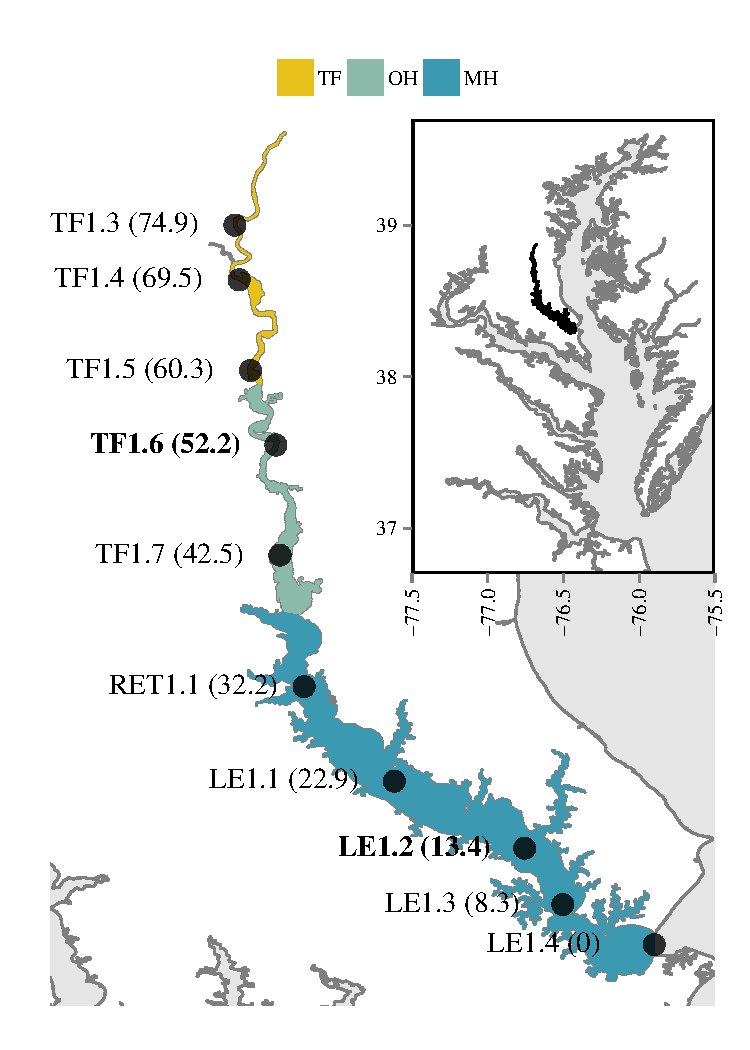
\includegraphics[width=0.7\textwidth]{figs/map-1} 

}

\caption{Patuxent River estuary with Chesapeake Bay inset. Fixed locations monitored by the Chesapeake Bay Program at monthly frequencies are shown along the longitudinal axis with distance from the mouth (km).  Study sites are in bold. Salinity regions in the Patuxent for the larger Chesapeake Bay area are also shown (TF = tidal fresh, OH = oligohaline, MH = mesohaline). See \cref{tab:statsum} for a numeric summary of station characteristics.}\label{fig:map}
\end{figure}



% chlorophyll trends by year, month, flow, combined
\begin{figure}[!ht]

{\centering 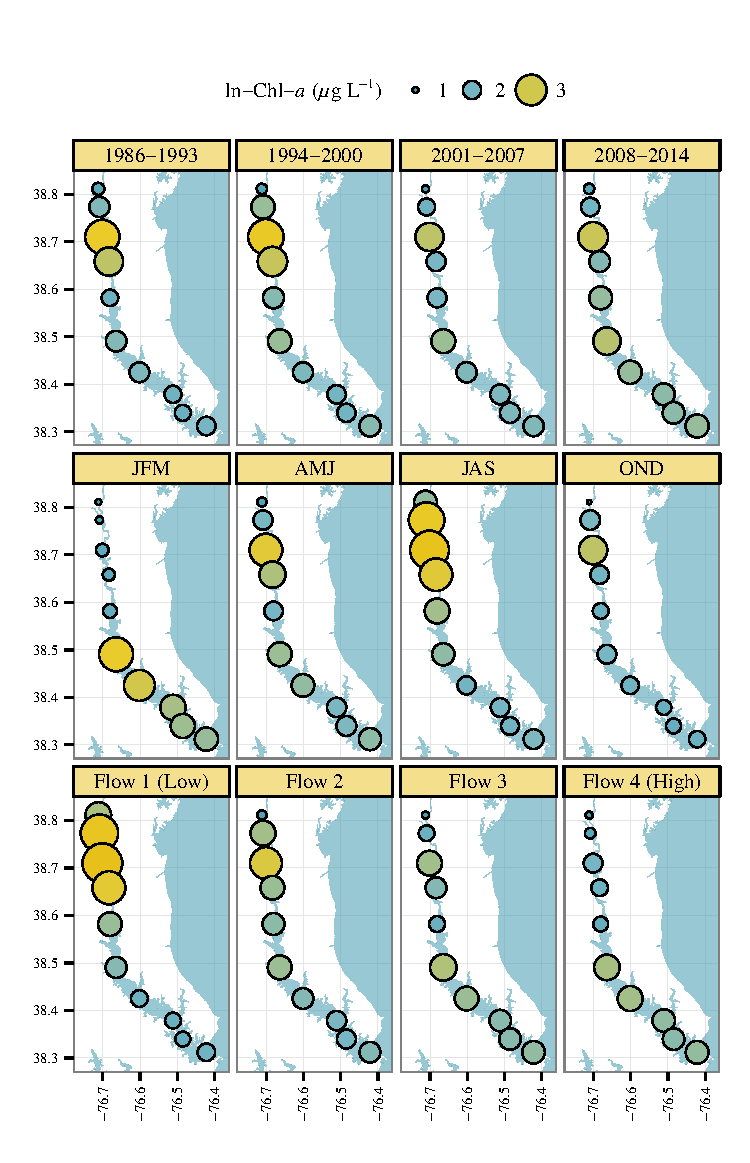
\includegraphics[width=\maxwidth]{figs/chlyrmofl-1} 

}

\caption{Annual, seasonal, and flow differences in chlorophyll trends at each monitoring station in the Patuxent River Estuary.  Size and color are proportional medians of ln-chlorophyll-a by year, season, and flow categories. See \cref{fig:map} for station numbers.}\label{fig:chlyrmofl}
\end{figure}



% predicted trends for each mod - monthly time series of observed with predictions, RMSE in fig


\begin{figure}
\centering
\subfloat[Monthly]{
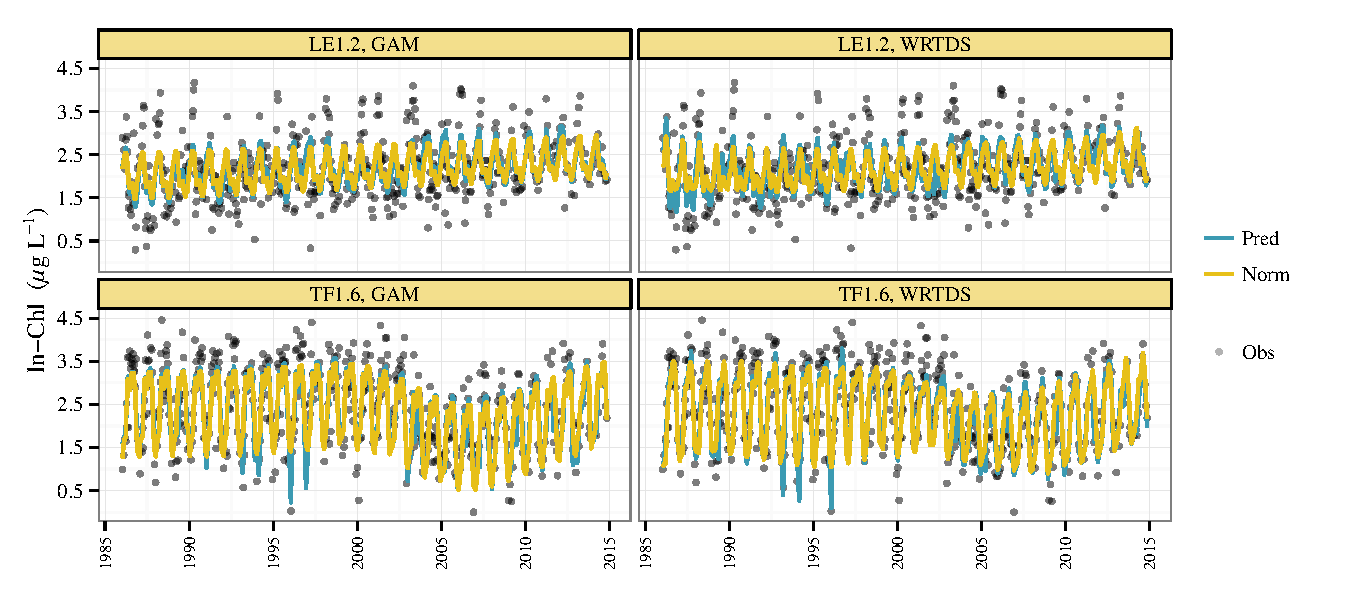
\includegraphics[width=\textwidth]{figs/predmo.pdf}
\label{fig:predmo}
}

\subfloat[Annual]{
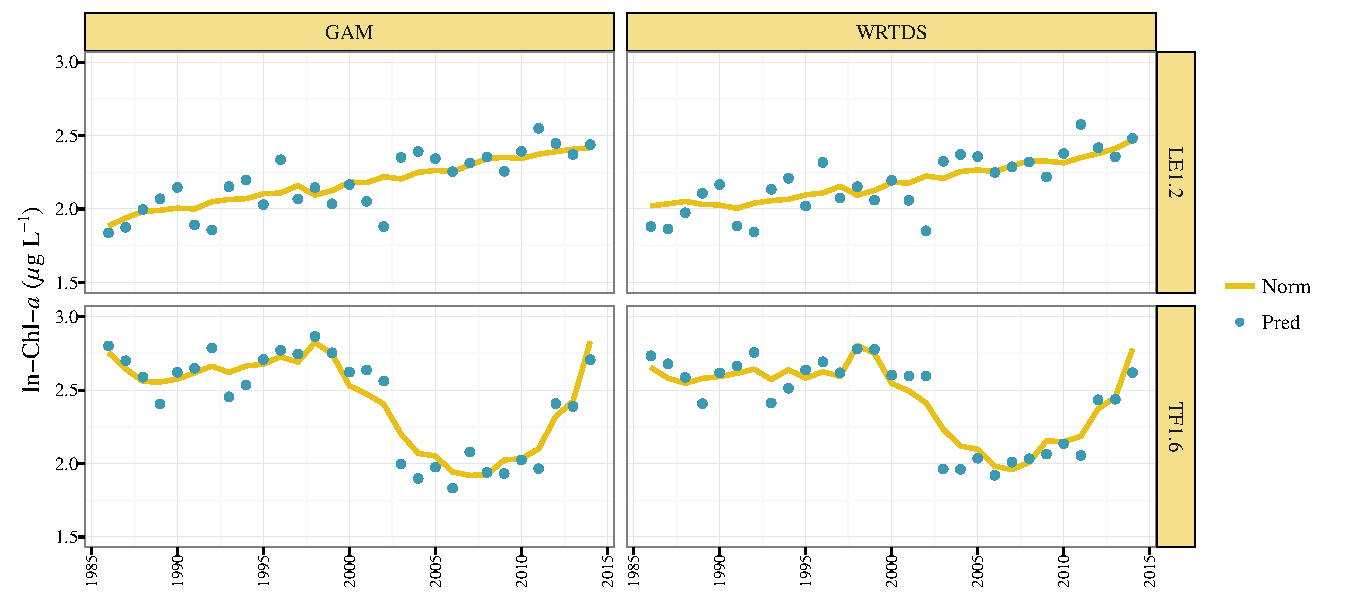
\includegraphics[width=\textwidth]{figs/predann.pdf}
\label{fig:predann}
}

\caption{Predicted chlorophyll from generalized additive models (GAM) and weighted regression (WRTDS) for LE1.2 and TF1.6 stations on the Patuxent River estuary.  \cref{fig:predmo} shows results at monthly time steps and \cref{fig:predann} shows results averaged by year.  Values in blue are model predictions and values in yellow are flow-normalized predictions.}
\label{fig:pred}
\end{figure}

% plot of seasonal variation from model predictions, by model and site, 
\begin{knitrout}
\definecolor{shadecolor}{rgb}{0.969, 0.969, 0.969}\color{fgcolor}\begin{figure}[!ht]

{\centering 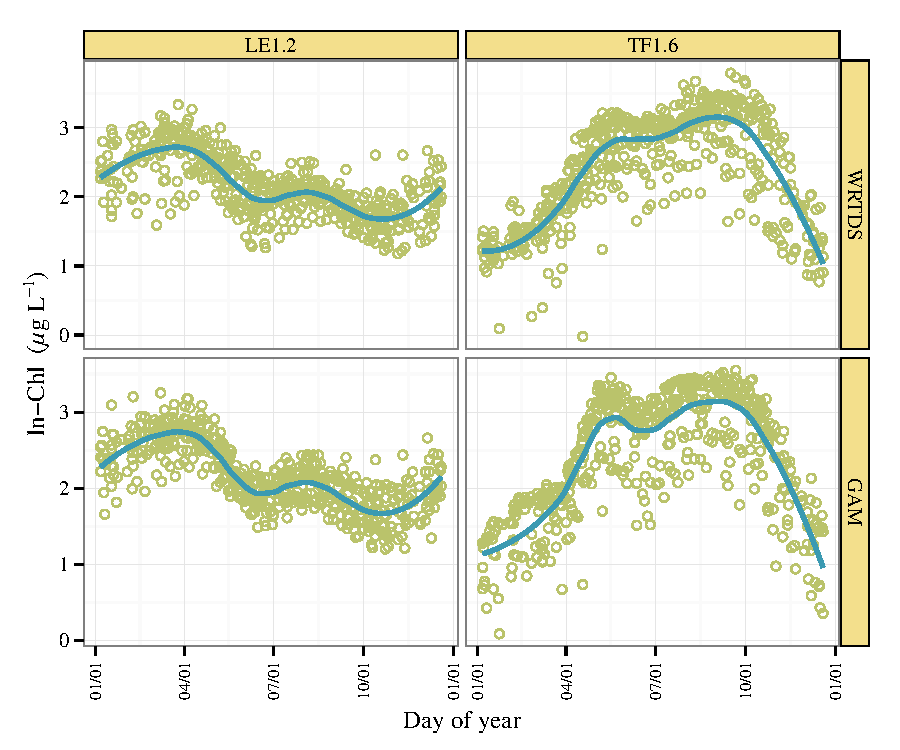
\includegraphics[width=\maxwidth]{figs/seas-1} 

}

\caption[Seasonal variation from observed and model predictions of \ac{chla} by station]{Seasonal variation from observed and model predictions of \ac{chla} by station.  Predictions are points by day of year from 1986 to 2014.  The blue line is a loess (locally estimated) polynomial smooth to characterize the seasonal components.}\label{fig:seas}
\end{figure}


\end{knitrout}

% wrtds v gam predictions by periods
\begin{figure}[!ht]

{\centering 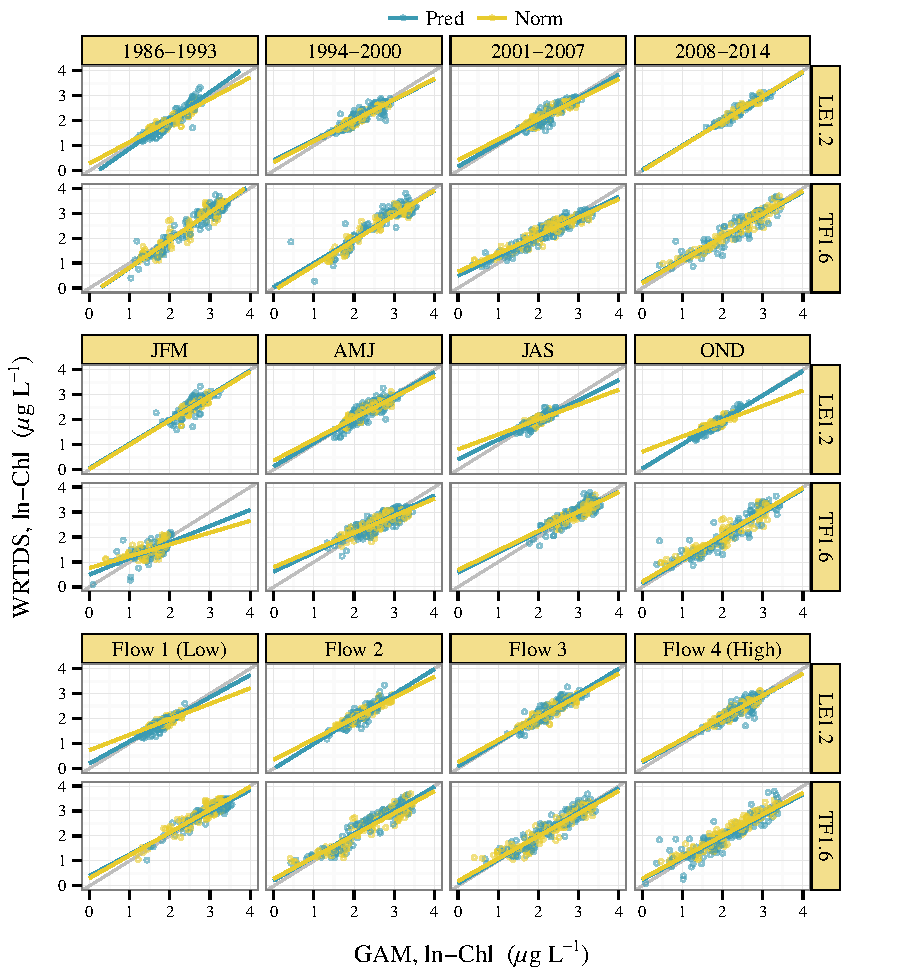
\includegraphics[width=\maxwidth]{figs/regprdnrm-1} 

}

\caption{Comparison of \ac{WRTDS} and \acp{GAM} results at each station (LE1.2, TF1.6) and different time periods.  Predicted and flow-normalized results are shown.  Time periods are annual groupings every seven years (top), seasonal groupings by monthly quarters (middle), and flow periods based on quantile distributions from the discharge record (low).  Regression lines for each model result and 1:1 replacement lines (thin grey) are also shown.  See \cref{tab:regprdnrm} for parameter estimates of regression comparisons.}\label{fig:regprdnrm}
\end{figure}



% dynaplots for each mod (as in Fig. 8 Beck and Hagy 2015)
\begin{figure}[!ht]

{\centering 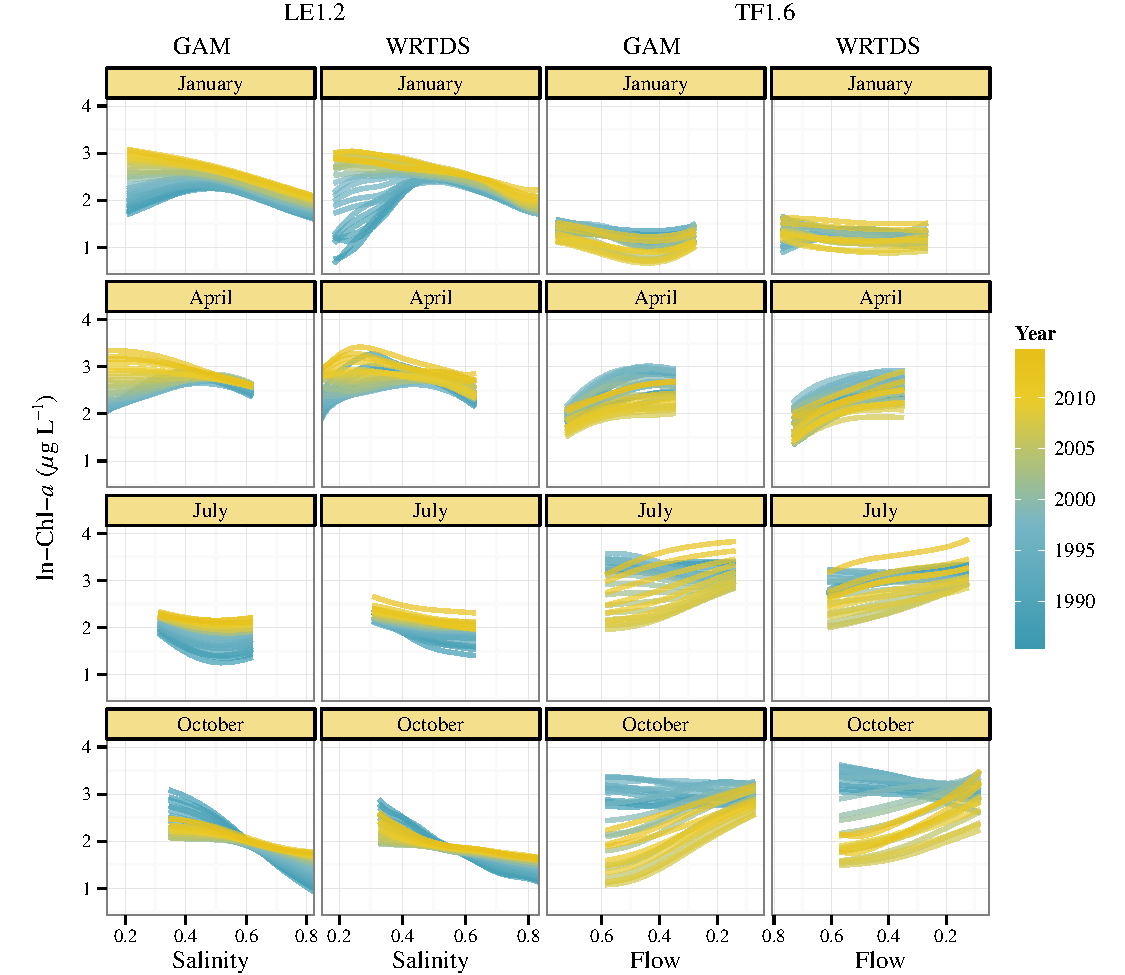
\includegraphics[width=1.02\textwidth]{figs/dynafig-1} 

}

\caption{Changes in the relationship between \ac{chla} and freshwater inputs (salinity decrease, flow increase) across the time series.  Separate panels are shown for each station (LE1.2, TF1.6), model type (GAM, WRTDS), and chosen months.  Changes over time are shown as different predictions for each year in the time series (1986 to 2014).  Salinity was used as a tracer of freshwater inputs at LE1.2, whereas the flow record at Bowie, Maryland was used at TF1.6.  The scales of salinity and flow are reversed for comparison of trends. Units are proportions of the total range in the observed data with values in each plot truncated by the monthly 5\textsuperscript{th} and 95\textsuperscript{th} percentiles.}\label{fig:dynafig}
\end{figure}



% examples of simulated datasets for eval of flow-normalization - daily, monthly, different flow effects
\begin{figure}[!ht]

{\centering 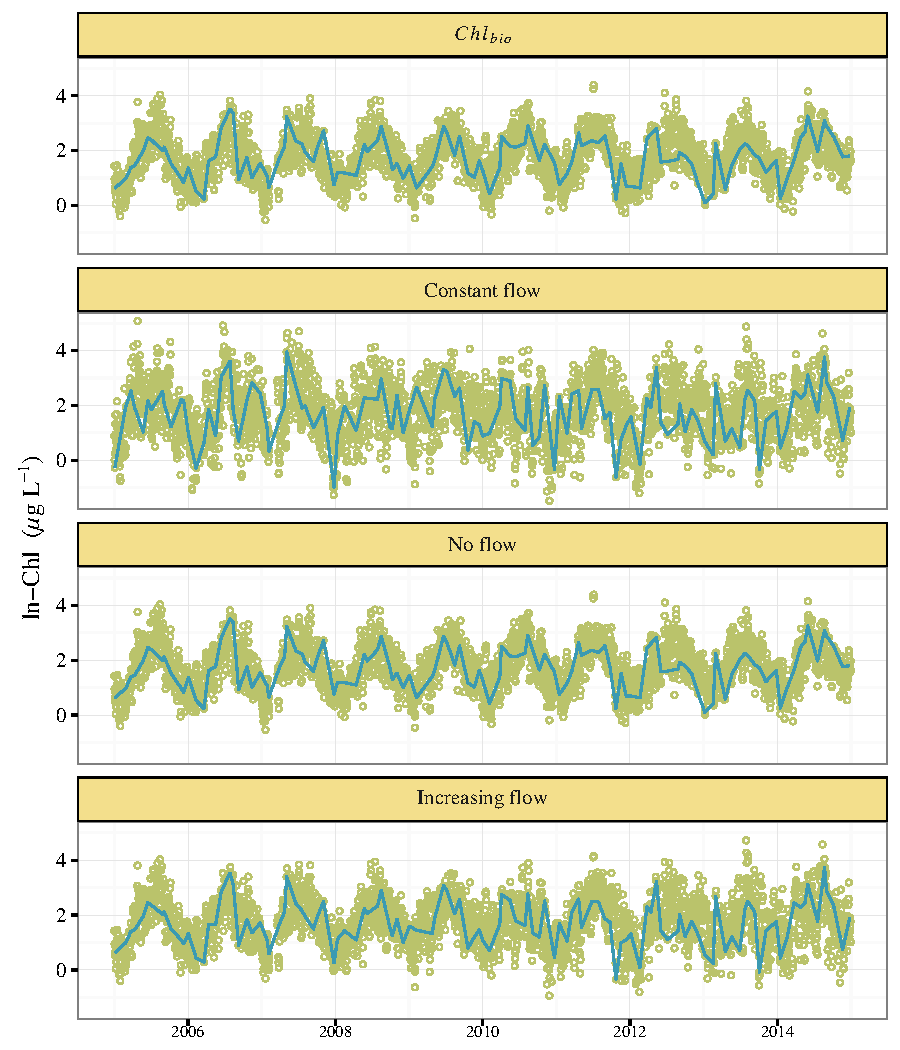
\includegraphics[width=\maxwidth]{figs/simex-1} 

}

\caption{Examples of simulated time series for evaluating flow-normalized results from \ac{WRTDS} and \acp{GAM}.  The plots show the simulated daily time series (points) and monthly samples (lines) from the daily time series used to evaluate the flow-normalized predictions from \ac{WRTDS} and \acp{GAM}.  From top to bottom, the time series show the biological \ac{chla} independent of flow and the three simulated datasets that represent different effects of flow: none, constant, and increasing effect.  The flow-normalized results for the simulated monthly time series from each model were compared to the first time series (biological chlorophyll) that was independent of flow.}\label{fig:simex}
\end{figure}



% dynaplot examples for mods with simulated data
\begin{figure}[!ht]

{\centering 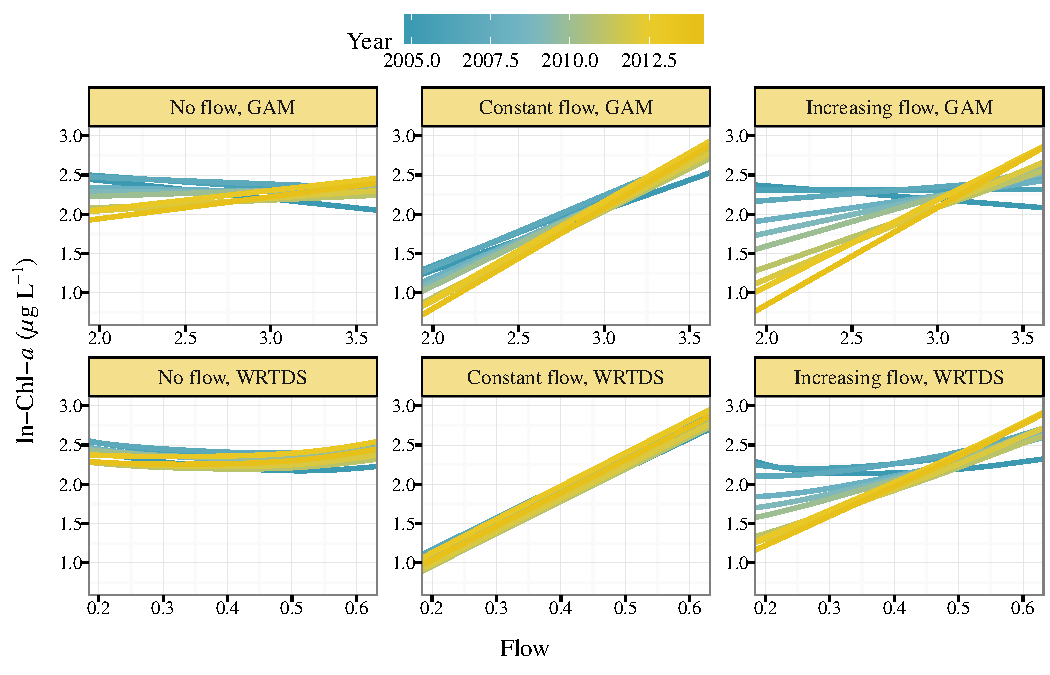
\includegraphics[width=\maxwidth]{figs/dynasim-1} 

}

\caption{Examples of changing relationships between \ac{chla} (\mugl) and flow (as proportion of the total range) over time (2005--2015) for each simulated time series in \cref{fig:simex}.  The plots are based on August predictions from three \ac{WRTDS} models for each time series to illustrate the simulated relationships between flow and chlorophyll.}\label{fig:dynasim}
\end{figure}



% results of flow-normalized data for simulations
\begin{figure}[!ht]

{\centering 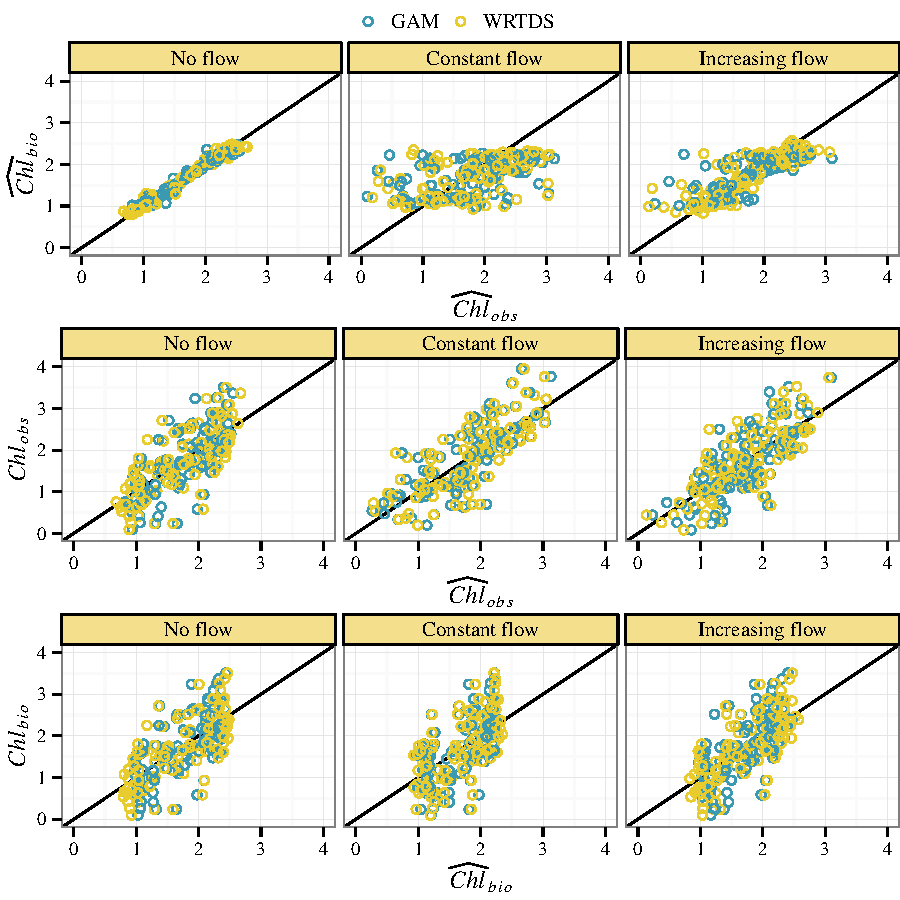
\includegraphics[width=\maxwidth]{figs/simres-1} 

}

\caption{Model predictions for three simulated datasets with different flow contributions (none, constant, increasing).  Estimated variables (e.g., $\widehat{Chl}_{bio}$) are compared to simulated variables (e.g., $Chl_{bio}$) to evaluate the ability of each model (\acp{GAM} and \ac{WRTDS}) to recreate the flow-normalized time series of chlorophyll (i.e., bottom plot, $\widehat{Chl}_{bio}$ vs $Chl_{bio}$) after removing a simulated flow component from the observed chlorophyll time series ($Chl_{obs}$).}\label{fig:simres}
\end{figure}



\end{document}
